%% FEUP THESIS STYLE for LaTeX2e
%% how to use feupteses (English version)
%%
%% FEUP, JCL & JCF, 31 July 2012
%%
%% PLEASE send improvements to jlopes at fe.up.pt and to jcf at fe.up.pt
%%

%%========================================
%% Commands: pdflatex tese
%%           bibtex tese
%%           makeindex tese (only if creating an index)
%%           pdflatex tese
%% Alternative:
%%          latexmk -pdf tese.tex
%%========================================

%% 2021-07-20: One-sided output by default
\documentclass[11pt,a4paper,numericrefs]{report}
%% For two-sided printing (for dead-tree output) comment previous line
%% and uncomment the next line
%% \documentclass[11pt,a4paper,twoside,openright]{report}

%% For iso-8859-1 (latin1), comment next line and uncomment the second line
\usepackage[utf8]{inputenc}
\usepackage{indentfirst}
\usepackage{amsfonts}
\usepackage{amsmath}
\usepackage{multirow}
\usepackage{booktabs}
\usepackage{tabularx}
\usepackage{floatrow}
% Table float box with bottom caption, box width adjusted to content
\newfloatcommand{capbtabbox}{table}[][\FBwidth]
%\usepackage[latin1]{inputenc}

%% English version

%% MEIC options
%\usepackage[meic]{feupteses}
%\usepackage[meic,juri]{feupteses}
%\usepackage[meic,final]{feupteses}
%\usepackage[meic,final,onpaper]{feupteses}

%% MEEC options
%\usepackage[meec]{feupteses}
%\usepackage[meec,juri]{feupteses}
%\usepackage[meec,final]{feupteses}

%% For other degrees
\usepackage{feupteses} % you must define the degree bellow
\usepackage{changepage}
\usepackage{subcaption}

%% Additional options for feupteses.sty: 
%% - onpaper: links are not shown (for paper versions)
%% - backrefs: include back references from bibliography to citation place

%% Uncomment to create an index (at the end of the document)
%\makeindex

%% Path to the figures directory
%% TIP: use folder ``figures'' to keep all your figures
\graphicspath{{figures/}}



%%========================================
%% Start of document
%%========================================
\begin{document}
%%----------------------------------------
%% TIP: if you want to define more macros, use an external file to keep them
%some macro definitions

% format
\newcommand{\class}[1]{{\normalfont\slshape #1\/}}

% entities
\newcommand{\Feup}{Faculdade de Engenharia da Universidade do Porto}

\newcommand{\svg}{\class{SVG}}
\newcommand{\scada}{\class{SCADA}}
\newcommand{\scadadms}{\class{SCADA/DMS}}



%%----------------------------------------

%%----------------------------------------
%% Information about the work
%%----------------------------------------
\title{GAN-based Anomaly Detection in Solar Wind Profiles}
\author{Ivo Saavedra}

%% Comment next line if not necessary for degree
\degree{Mestrado em Engenharia Informática e Computação}

%% Uncomment next line for date of submission
%\thesisdate{July 31, 2008}

%% Comment next line copyright text if not used
\copyrightnotice{Ivo Saavedra, 2023}

\supervisor{Supervisor}{André Restivo}

%% Uncomment next line if necessary
\supervisor{Co-Supervisor}{Filipa Barros}

%% Uncomment committee stuff in the final version if used
%\committeetext{Approved by \ldots:}
%\committeemember{President}{Name of the President}
%\committeemember{Referee}{Name of the Referee}
%\committeemember{Referee}{Name of the Referee}

%% Uncomment signature line in the final on paper version if used
%\signature

%% Specify cover logo (in folder ``figures'')
\logo{uporto-feup.pdf}

%% Uncomment next line for additional text below the author's name (front page)
%\additionalfronttext{Preparação da Dissertação}

%%----------------------------------------
%% Preliminary materials
%%----------------------------------------

% remove unnecessary \include{} commands
\begin{Prolog}
  \chapter*{Resumo}
%\addcontentsline{toc}{chapter}{Resumo}

A Ciência do Clima Espacial é um campo de pesquisa vital que visa compreender as condições na superfície do Sol, que podem afetar negativamente a vida na Terra. Apesar de ser um campo bem desenvolvido, as condições que levam a essas fenómenos nefastos ainda não são totalmente compreendidas. Esta limitação é principalmente atribuída à dificuldade em obter dados de alta qualidade da superfície do Sol.

De forma a contornar este problema, alguns modelos de simulação tentam extrapolar as condições no Sol analisando dados de outras medições. Um exemplo disso é o MULTI-VP que usa magnetogramas de várias fontes (por exemplo, Wilcox Solar Observatory) e determina a estrutura do campo magnético de fundo do vento solar. No entanto, essas simulações demoram muito tempo a convergir e requerem estimativas iniciais de especialistas, feitas manualmente. Recentemente, uma abordagem baseada em Machine Learning foi projetada para atenuar esses problemas. Esta removeu a necessidade de estimativas iniciais, prevendo automaticamente as condições iniciais da simulação. Além disso, provou que pode haver uma redução significativa no tempo de execução do simulador. Apesar disso, os modelos de previsão ainda não são robustos o suficiente para serem usados em aplicações do mundo real. Como em muitos outros problemas de Machine Learning, acreditamos que a presença de anomalias no conjunto de dados de treino tenha prejudicado a sua performance.

Uma possível teoria é que as condições iniciais estão diretamente correlacionadas com o tempo de computação da simulação, e que melhores estimativas inicias levam a tempos de execução do MULTI-VP mais rápidas. Posto isto, nesta dissertação, aplicamos vários métodos de clustering e de deteção de anomalias de forma a melhorar a qualidade das condições iniciais e verificar se isso resultava em simulações mais rápidas do MULTI-VP.

Vários métodos de clustering foram testados nos dados de magnetogramas usados no treino do modelo de previsão, para determinar qual seria o mais apropriado. Adicionalmente, um conjunto de métodos de treino baseados nas técnicas de clustering foram testados, dos quais pelo menos um gerou estimativas mais próximas às previsões da simulação. Apesar disto, não houve qualquer redução no tempo de execução da simulação.

Para melhorar os resultados dos experimentos anteriores, vários métodos de detecção de anomalia adversária foram testados. Os modelos foram retreinados sem as anomalias detectadas o que resultou em piores condições de fluxo inicial quando
comparado ao resultado final do MULTI-VP; no entanto, o tempo de computação foi ligeiramente menor do que na implementação anterior.

Concluindo, os resultados das experiências com os métodos de clustering e de deteção de anomalias adversariais parecem indicar que o desempenho do simulador não está correlacionado com a proximidade das condições iniciais às soluções da simulação.

% Com o fim de melhorar os resultados das experiências anteriores, vários métodos de aprendizagem adversarial foram implementados e testados. Os modelos de previsão treinados com os métodos de clustering sofreram um novo processo de treino sem os dados anomalos no dataset de treino. Isto resultou em piores condições iniciais quando comparado com as estimativas finais da simulação. Contudo, a simulação demorou menos tempo a alcançar um solução viável do que com as condições iniciais dos modelos anteriores.

% Podemos classificar os outliers como dados fora da distribuição, anomalias, novidades e desvios. Estes podem ser causados por falhas de sistema, ruído de sensor, erros humanos e operações maliciosas. Mais recentemente, GANs têm provado ser métodos eficazes de deteção de anomalias de maneiras não supervisionadas.

% Com isto, esta dissertação propõe uma abordagem baseada em GANs para deteção de outliers em perfis de vento solar que depois serão usados para treinar um modelo de previsão. O impacto do novo método será avaliado em relação aos resultados obtidos através de um modelo de previsão treinado com dados não normalizados.

% Vários métodos de deteção de anomalias baseados em GANs foram estudados para determinar qual se adequava melhor ao problema. Com as lições aprendidas neste passo, propusemos uma metodologia que incorpora GANs para deteção de amostras de perfis de vento solar anómalos nos dados usados para treinar modelos para estimativa de condições iniciais. Um método de treino foi projectado, juntamente com um mecanismo de detecção de anomalias. Os critérios de avaliação da metodologia proposta também foram definidos.
\vspace{1cm}
\textbf{Palavras-chave:} Meteorologia Espacial, Vento Solar, Aprendizagem Computacional, Clustering, Deteção Adversarial de Anomalias


\chapter*{Abstract}
%\addcontentsline{toc}{chapter}{Abstract}
Space Weather Science is a vital field of research that aims to understand the conditions on the Sun's surface, which can negatively impact life on Earth. Despite being a well-researched field, the conditions that lead to these phenomena are still not fully understood. This limitation is mainly attributed to the difficulty in acquiring high-quality data from the Sun's surface.

To circumvent this issue, some simulation models try to extrapolate the conditions on the Sun by analyzing data from other measurements. An example of this is MULTI-VP which uses magnetograms from various sources (\textit{e.g.}, Wilcox Solar Observatory) and determines the structure of the solar wind's background magnetic field. However, these simulations take a long time to converge and require initial expert estimations, which are handmade. Recently, a machine learning approach has been designed to attenuate these issues. It removed the need for initial estimates by automatically predicting the starting conditions of the simulation. In addition, it has shown that there can be a significant reduction in the execution time of the simulator. Despite this, given their lack of physical cohesion, the prediction models are still not robust enough for real-world applications. 

We posit that initial conditions directly influence the computation time of the simulation and that better initial estimates will lead to faster executions. Thus, in this dissertation, we applied clustering and anomaly detection techniques to improve the quality of the initial conditions and determine if this would lead to faster MULTI-VP executions.

Several clustering experiments were conducted on the available magnetogram dataset to determine the best-suited clustering method. In addition, various clustering-based approaches for enhancing the prediction model were tested, with the selected method producing initial flow conditions closer to the simulation outputs. Despite this, there was no reduction in the computation time of the simulation.

To improve the previous experiments' results, various adversarial anomaly detection methods were designed and tested. The prediction models of the clustering-based experiments were retrained without the detected anomalies and resulted in worse initial flow conditions when compared to the final output of MULTI-VP; however, this time, the computation time was slightly lower than on the previous implementation.

In conclusion, the experiments conducted in this dissertation seem to indicate that the performance of the MULTI-VP simulator is not directly linked to the initial flow condition's approximation to the final solutions.



% Thus, this dissertation aims to apply GANs to detect anomalies in solar wind profiles to measure
% their influence on the already developed prediction models. This will be done by taking
% advantage of the discriminative and generative abilities of GANs. In addition, we will also evaluate the impacts of the improved prediction models, trained with normalized datasets, on the performance of the simulation.

% Several GAN-based anomaly detection methods were studied to determine which suited the problem. With the insights from this step, we proposed a methodology incorporating GANs for detecting anomalous solar wind profile samples in the data used to train models for initial condition estimation. A training method was presented along with an anomaly detection mechanism. Additionally, the evaluation criteria for the proposed methodology were also defined.

% TODO conclusion
\vspace{1cm}
\noindent\textbf{Keywords:} Space Weather, Solar Wind, Machine Learning, Clustering, Adversarial Anomaly Detection % the abstract
  % \chapter*{Agradecimentos}
%\addcontentsline{toc}{chapter}{Agradecimentos}

Aliquam id dui. Nulla facilisi. Nullam ligula nunc, viverra a, iaculis
at, faucibus quis, sapien. Cum sociis natoque penatibus et magnis dis
parturient montes, nascetur ridiculus mus. Curabitur magna ligula,
ornare luctus, aliquam non, aliquet at, tortor. Donec iaculis nulla
sed eros. Sed felis. Nam lobortis libero. Pellentesque
odio. Suspendisse potenti. Morbi imperdiet rhoncus magna. Morbi
vestibulum interdum turpis. Pellentesque varius. Morbi nulla urna,
euismod in, molestie ac, placerat in, orci. 

Ut convallis. Suspendisse luctus pharetra sem. Sed sit amet mi in diam
luctus suscipit. Nulla facilisi. Integer commodo, turpis et semper
auctor, nisl ligula vestibulum erat, sed tempor lacus nibh at
turpis. Quisque vestibulum pulvinar justo. Class aptent taciti
sociosqu ad litora torquent per conubia nostra, per inceptos
himenaeos. Nam sed tellus vel tortor hendrerit pulvinar. Phasellus
eleifend, augue at mattis tincidunt, lorem lorem sodales arcu, id
volutpat risus est id neque. Phasellus egestas ante. Nam porttitor
justo sit amet urna. Suspendisse ligula nunc, mollis ac, elementum
non, venenatis ut, mauris. Mauris augue risus, tempus scelerisque,
rutrum quis, hendrerit at, nunc. Nulla posuere porta orci. Nulla dui. 

Fusce gravida placerat sem. Aenean ipsum diam, pharetra vitae, ornare
et, semper sit amet, nibh. Nam id tellus. Etiam ultrices. Praesent
gravida. Aliquam nec sapien. Morbi sagittis vulputate dolor. Donec
sapien lorem, laoreet egestas, pellentesque euismod, porta at,
sapien. Integer vitae lacus id dui convallis blandit. Mauris non
sem. Integer in velit eget lorem scelerisque vehicula. Etiam tincidunt
turpis ac nunc. Pellentesque a justo. Mauris faucibus quam id
eros. Cras pharetra. Fusce rutrum vulputate lorem. Cras pretium magna
in nisl. Integer ornare dui non pede. 

\vspace{10mm}
\flushleft{O Nome do Autor}
  % the acknowledgments
  % \cleardoublepage
\thispagestyle{plain}

\vspace*{8cm}

\begin{flushright}
   \textsl{``You should be glad that bridge fell down. \\
           I was planning to build thirteen more to that same design''} \\
\vspace*{1.5cm}
           Isambard Kingdom Brunel
\end{flushright}
    % initial quotation if desired
  \cleardoublepage
  \pdfbookmark[0]{Table of Contents}{contents}
  \tableofcontents
  \cleardoublepage
  \pdfbookmark[0]{List of Figures}{figures}
  \listoffigures
  \cleardoublepage
  \pdfbookmark[0]{List of Tables}{tables}
  \listoftables
  \chapter*{Abbreviations}
%\addcontentsline{toc}{chapter}{Abbreviations}
\chaptermark{ABREVIATURAS E SÍMBOLOS}

\begin{flushleft}
\begin{tabular}{l p{0.8\linewidth}}
GAN      & Generative Adversarial Network\\
CME      & Coronal Mass Ejection\\
NN      & Neural Network\\
CNN     & Convolutional Neural Network

\end{tabular}
\end{flushleft}

  % the list of abbreviations used
\end{Prolog}

%%----------------------------------------
%% Body
%%----------------------------------------
\StartBody

%% TIP: use a separate file for each chapter
\chapter{Introduction} \label{chap:intro}

The Sun continuously releases a stream of particles known as \textit{solar wind}. This stream consisting of high-velocity charged particles (e.g. protons and electrons) can reach planetary surfaces unless thwarted by an atmosphere, magnetic field, or both. In Earth's case, the magnetosphere and the atmosphere, to a smaller extent, block out most of the radiation emitted by the Sun. However, other more extreme events like solar flares and CMEs (Coronal Mass Ejections) can provoke negative effects on the Earth's surface and upper atmosphere. 

These events can impact the Earth in three primary ways. Firstly, they can cause radio blackouts that predominantly affect satellites and, consequently, geolocation and communication systems. Secondly, solar radiation storms can endanger astronauts and spacecraft orbiting the Earth. Lastly, the most severe of these events are geomagnetic storms, which have historically caused significant disturbances. Examples of such disturbances include the Carrington Event in 1859 and a geomagnetic storm that affected Quebec's power grid in 1989\footnote{List of solar storms: \url{https://en.wikipedia.org/wiki/List_of_solar_storms}}.

Space Weather Science is a field that aims to prevent the consequences of such events; however, the factors that result in their formation are still not fully understood. Some simulation models have been designed to try and fill this gap \cite{pinto.rouillard_MultipleFluxtubeSolar_2017, odstrcil.pizzo_ThreedimensionalPropagationCoronal_1999}, but they require initial expert guesses. Recently, an ML (Machine Learning) model has been developed \cite{barros_InitialConditionEstimation_} to improve these initial predictions based on known data. Like other ML problems, the quality of the predictions is very dependent on the quality of the training data.

%The field of \textit{Space Weather Science} emerged with the aim of understanding the formation of the phenomena that could affect Earth, in order to implement early warning systems. Despite this being a well-developed field of science, the correlations between the Sun's structures and these phenomena are not yet fully formulated and their prediction is mostly speculative. Several simulations have been developed to try and fill this gap (e.g. MULTI-VP \cite{pinto.rouillard_MultipleFluxtubeSolar_2017}). These models require initial estimations before starting the simulation and their performance is affected by the quality of these initial values.

%Several simulation models have been developed recently to try and estimate these conditions with data collected from satellites, probes and observatories. 

\section{Motivation} \label{sec:motivation}
In 1859, Carrington recorded the first and largest known solar flare in history, which is now commonly referred to as the Carrington event. This phenomenon was so extreme that it caused geomagnetic storms in unexpected latitudes and provoked fires on telegraph wires.  Carrington was also able to correlate the event with a geomagnetic storm that occurred several hours later. His pioneering work is widely recognized as the inception of the scientific discipline known as Space Weather \cite{schwenn_SpaceWeatherSolar_2006}.

The field of \textit{Space Weather Science} emerged with the aim of understanding the formation of phenomena that could affect Earth to evaluate their effects and to create early warning systems. Despite significant advancements in this scientific field, the correlations between the Sun's structures and these phenomena are not yet fully formulated and are mostly speculative.  For instance, it is still unknown why the atmosphere of the Sun is considerately hotter than its surface. The main leading theory is that the magnetic field transports energy deep from the convection zone through the surface and up to the atmosphere. It is also posited that the magnetic fields on the surface sometimes collide, provoking large explosions and therefore causing the atmosphere to heat even further. Another enigma is the acceleration of the solar wind (up to millions of miles) out of the corona. Some correlation between the magnetic field and solar wind acceleration has been found; however, the effect remains a mystery.

The answer to questions like these can contribute to a greater understanding of the underlying processes of the Sun that influence solar weather. Consequently, predicting future events that could impact the Earth, satellites, and space stations orbiting it would become easier. Thus far, these answers have been delayed by the technological limitations on measuring solar events. In 2018, NASA's Parker Solar \footnote{Parker Solar Probe: Humanity’s First Visit to a Star \url{https://www.nasa.gov/content/goddard/parker-solar-probe-humanity-s-first-visit-to-a-star}} probe was launched on a mission to orbit the Sun's, to understand the acceleration of solar wind at the corona. More recently, ESA launched the Solar Orbiter to measure the solar wind and record images of the uncharted polar regions, closer than every other solar probe\footnote{ESA: Solar Orbiter \url{https://www.esa.int/Science_Exploration/Space_Science/Solar_Orbiter}}. The PUNCH\footnote{NASA Selects Missions to Study Our Sun, Its Effects on Space Weather \url{https://www.nasa.gov/press-release/nasa-selects-missions-to-study-our-sun-its-effects-on-space-weather}} mission was launched to try and shed some light on the formation of the solar wind on the Sun's surface.

MHD (magnetohydrodynamic) simulators like MULTI-VP \cite{pinto.rouillard_MultipleFluxtubeSolar_2017} and ENLIL \cite{odstrcil.pizzo_ThreedimensionalPropagationCoronal_1999}, were developed in order to try and extrapolate coronal conditions from limited observations of solar events from probes and observatories. The execution of these simulations relies on initial estimations, usually performed by hand after an analysis of the data (a very time-consuming task). Additionally, it has been posited that good initial estimations have the potential to reduce the simulation's execution time significantly. The process of making the initial predictions as well as the extensive execution time of the simulations make it difficult to create early warning systems that can prevent the effects of solar events on Earth.

\section{Problem Definition} \label{sec:prob_definition}
The exponential growth of data acquisition has presented a significant challenge in promptly analyzing the vast amount of available information. The sheer amount of data is becoming increasingly hard for researchers to process, especially on data linked to near-real-time utilization. Machine learning has become one of the main methods of evaluating the data efficiently for problems associated with space weather prediction. However, most deep learning models are very susceptible to large variations in the data that can severely decrease the performance of these models. The anomalies can originate from the instrument and detector noise, statistical noise from the small flux of photons, and external noise may include instrumentation jitter, stray starlight, and cosmic ray background \cite{anirudh2022ReviewDataDriven2022}.

Recently, a NN \cite{barros_InitialConditionEstimation_} was developed to perform initial estimations for solar wind profiles that would later be fed to MULTI-VP \cite{pinto.rouillard_MultipleFluxtubeSolar_2017}. This reduced the time needed to generate the initial estimations required by the simulation, which were previously done by hand. Additionally, it was observed that producing initial estimates closer to the final simulation reduced the computation time of the simulation, with a mean speedup of 1.06. Despite this, it was concluded that the prediction model was not producing the best possible estimates. On one hand, this might have been because the model managed to learn the most concentrated observations and failed to learn the ones in the peripheries. Another possibility is that the existence of anomalies in the dataset was hindering the performance of the model resulting in worse estimates.

The problem addressed in this thesis is to enhance the quality of the training data, which is then to be used for predicting initial conditions associated with solar wind behaviour.

\section{Goals}\label{sec:goals}
This thesis aims to enhance the prediction ability of the neural network \cite{barros_InitialConditionEstimation_} responsible for generating initial predictions for solar wind formations. With this, we aim to produce closer initial condition estimations to MULTI-VP's \cite{pinto.rouillard_MultipleFluxtubeSolar_2017} final estimates. We intend to achieve this by:

\begingroup
    \renewcommand\labelenumi{(\theenumi)}
    \begin{enumerate}
    \item applying clustering techniques in the training of the models for initial condition prediction so these can better capture the features of the data;
    \item applying adversarial anomaly detection techniques to detect and filter faulty measurements in the data used to train the prediction models.
\end{enumerate}
\endgroup


As a consequence of better initial condition estimations, we intend to reduce the computation time that the simulation takes to reach a viable solution.



% The objective of this thesis is to take advantage of GANs' generative and discriminative abilities to identify anomalous input data within solar wind profiles. The  identified anomalous data points will be excluded  from the input provided to a neural network (NN) model \cite{barros_InitialConditionEstimation_} responsible for generating initial predictions for solar wind formation. This approach aims to improve the accuracy of the NN model's predictions and, consequently, reduce the computation time required by MULTI-VP \cite{pinto.rouillard_MultipleFluxtubeSolar_2017} to generate feasible solutions.

% The developed architecture should be able to generate new solar wind profiles similar to the real distribution and to correctly detect samples that fall out of that distribution.
\clearpage
\section{Document Structure}\label{sec:doc_struct}
This first chapter has provided the context for the problem addressed in this dissertation. The remaining sections of the document are organized as follows:

\begin{itemize}
    \item Chapter \ref{chap:background}, explains the background needed to understand the current problems in the area of space weather science. Some concepts related to neural networks and anomalies are also introduced to provide a basis for methods discussed in the remainder of the document.

    \item Chapter \ref{chap:sota}, provides an analysis o fthe current state-of-the-art methods for clustering and adversarial anomaly detection.

    \item Chapter \ref{chap:research_proposal}, goes into more depth on the problem this thesis aims to solve and the approach that will be taken.

    % \item Chapter \ref{chap:eda}, explains the dataset that will be used throughout this thesis.

    \item Chapter \ref{chap:clustering} explains the clustering methods used on the dataset, followed by the experiments and discussion of the results.

    \item Chapter \ref{chap:aad} starts by explaining the origins of adversarial learning and the experiments undertaken with this type of approach, followed by a brief discussion of the results.

    \item Chapter \ref{chap:remarks} evaluates this thesis's hypothesis and provides a brief conclusion for the work carried out.
\end{itemize}

% hipotese - retirar outliers para o processo de aprendizagem ser melhor 
\chapter{Background}\label{chap:background}
In this chapter, a basic introduction to solar weather and the main events associated with it will be presented. Additionally, a brief explanation of the Machine Learning (ML) terms that are needed in the context of this dissertation will be provided.

\section{Space Weather}
"Space weather refers to the dynamic, highly variable conditions in the geospace environment, including those on the Sun, in the interplanetary medium, and in the magnetosphere-ionosphere-thermosphere system. Adverse changes in the near-Earth space environment can diminish the performance and reliability of both spacecraft and ground-based systems." (\cite{BAKER19987})

\subsection{Solar Phenomena}\label{sec:solar_events}
The increasing dependence on technologies vulnerable to solar weather conditions has made it increasingly important to detect incidents, like the Carrington event \cite{schwenn_SpaceWeatherSolar_2006}, that would significantly damage assets on Earth beforehand. In this section, a brief introduction to these phenomena will be provided.\\

\noindent\textbf{Sunspots.} These structures consist of dark central regions (umbra), which are colder than the rest of the Sun's surface, and more luminous external regions (penumbra). Sunspots are known to be regions with strong magnetic fields (1000 times stronger than in the surrounding normal surface). It is theorized that these magnetic fields interfere with the convection of the Sun, effectively cooling the regions where they appear. Sunspots often originate as groups concentrated in specific areas of the Sun, and their frequency and size vary with the 11-year solar cycle \cite{moldwin_2008}. \\


\noindent\textbf{Coronal Mass Ejections (CME).} These events are best described as mass ejections of plasma into space after solar eruptions. It is posited that their formation occurs mainly from magnetic reconnection, which occurs when magnetic field lines collide and realign into a new configuration (releasing large amounts of energy). After their formation, CMEs can expand through space to great distances and collide with planetary atmospheres. The effects on Earth include geomagnetic storms, damage to electronics on orbiting satellites, endangerment of astronauts or planes, damage to electrical grids and disruption of radio communication. Due to their length (at least 0.25AU), CMEs can take over a day to pass Earth. While slower CMEs can take days before reaching Earth, the fastest ones arrive in approximately 15-18 hours. \cite{priest_2014, moldwin_2008}.\\

\noindent\textbf{Solar Flares.} These events are often characterized as intense and temporary releases of energy that blast large amounts of charged particles into space. Flares are known to last only a few minutes and reach temperatures of 100 million K, much higher than the ones at the core of the Sun. Like CMEs, flare formations are associated with energy releases from magnetic reconnection and are primarily concentrated in the Sun's active regions. Flares are almost always associated with CMEs, but can also occur separately from them. Flares can be classified as A, B, C, M or X based on the X-ray flux measurements on Earth by the GOES spacecraft\footnote{GOES overview and history \url{https://www.nasa.gov/content/goes-overview/index.html}} \cite{moldwin_2008, priest_2014}.\\

\noindent\textbf{Solar Wind.} This phenomenon results from plasma's constant expulsion and expansion into interplanetary space. More concretely, the solar wind consists of mostly protons, helium nuclei and electrons that move away from the Sun at supersonic speeds and carry the Sun's magnetic field with it. It streams away from the Sun at different velocities, which allows for it to be classified as fast (700 to 750 $km s^{-1}$) or slow (300 to 400 $km s^{-1}$). The latter usually occurs on the Sun's equatorial line, and the former is concentrated in open magnetic field regions of the Sun. The exact originating factors for the slow solar wind are still unknown; however, for fast solar wind, it is known that its origin is coronal holes. The solar wind has as properties (at 1 AU) a velocity of 400 $km s^{-1}$, a temperature of 1 million K, and a density of 5 particles $cm^{-3}$ \cite{moldwin_2008, priest_2014}.

\subsection{Magnetohydrodynamic Simulation Models}\label{sec:back_mhd_sim}
The reasons for the acceleration of solar wind are mainly attributed to thermal heating; however, this does not explain the high speeds it reaches. The additional acceleration is often attributed to the magnetic field, but no physical model can currently explain the correlation. Similarly, the origins of the solar wind are mostly unknown, especially for slow solar wind compared to fast solar wind \cite{priest_2014}.

These difficulties are mostly attributed to the absence of sensitive, high-resolution coronal magnetic field measurements that do not allow for a full explanation of coronal physics. The limitations in this field make it more challenging to comprehend solar events like CMEs and the acceleration of the solar wind \cite{solanki.etal_SolarMagneticField_2006}.

To try and fill these gaps in Space Weather Science, several magnetohydrodynamic (MHD) models have been developed to try and give an answer to these questions. These models compute numerically intensive problems based on MHD equations. For this, they require the definition of appropriate boundaries and initial state definitions. Due to their complexity, MHD models often focus on single events and introduce assumptions and simplifications for the surrounding phenomena. For this reason, the research community has developed relatively simple MHD models to describe complex processes in the past decades.
%\section{Machine Learning}\label{sec:ml}
%Machine learning (ML) is a branch of artificial intelligence (AI) and computer science which focuses on the use of data and algorithms to imitate the way that humans learn, gradually improving its accuracy\footnote{What is machine learning? \url{https://www.ibm.com/cloud/learn/machine-learning}}.

\section{Neural Networks}\label{sec:nn}
Neural Networks (NN) or Artificial Neural Networks (ANNs) are one of the main ML models. Biological neural networks from animal brain structures inspire their design. NNs consist of a set of node layers, the input layer, one or more hidden layers and the output layer. Each node is loosely connected to other nodes, each with its associated weights and threshold values. The connections between the nodes are called edges, allowing for communication between nodes and also having their associated weights. Signals travel from the input layer through the hidden layers to the output layer. If a given node's output is higher than its associated threshold value, it is activated and sends data to the next layer.

\subsection{Deep Neural Networks}\label{sec:deep_learning}
Deep Neural Networks (DNNs) derive from the  deep learning subfield of ML and are based on NNs. Their distinguishing factor from previous methods is representation learning (also known as feature learning) with multiple levels of abstraction. This technique allows models to discover the underlying data structures needed for feature detection and classification. These methods have been successfully applied in speech recognition, visual object recognition and detection, among others (\cite{lecun.etal_DeepLearning_2015}). The term "deep" comes from a large number of stacked layers that the model has compared to normal NNs. The most basic features are learned in the starting layers and the most complex at the bottom layers. DNNs usually have a feed-forward architecture where the data flows from the top layers to the output layer. In the end, the errors are back-propagated through the network to adjust the weights of the nodes in each layer.

\subsection{Autoencoders}
Autoencoders (AE) are a subtype of neural networks, and their main purpose is to compress existing data into meaningful representations, which are then decompressed back to the original input. Examples of applications include classification, clustering, anomaly detection (oftentimes adversarially trained), dimensionality reduction, and others. Its objective is to minimize the distance between the reconstructed and original samples. Therefore, the training goal is to minimize the loss function  
\begin{equation}
    L(\theta, \phi) = \mathbb{E}_{x\sim\mu_{ref}}[d(x, D_{\theta}(E_{\phi}(x))]
    \label{eq:ae_objective_func}
\end{equation} where $\theta$, $\phi$ are the parameters of the encoder, $E_\theta$ and the decoder $D_\phi$, respectively; $x$ is the original sample, $\mu_{ref}$ is the reference probability distribution and $d$ is the distance function that measures the reconstruction quality by comparing $x$ with its reconstructed examples, $D_{\theta}(E_{\phi}(x)$.

Regularizations are often applied to objective functions in line with the application of the autoencoder or to avoid overfitting. Some methods purposely reduce the reconstruction ability of the autoencoder to produce more meaningful compressions and vice versa. Possible variations of AEs include \textit{Sparse AEs}, which aims to reduce the dimensionality of the input data, \textit{Denoising AEs}, mainly used to reduce noise in images and \textit{Contracting AEs}, which aims to reduce the number of features that need to be learned by removing the unnecessary ones. %TODO cite

%A significant improvement over traditional AEs, known as Variational Autoencoders (VAE) was created by \cite{}. Its main goal is to defined with a greated degree of precision the distribution of the encoded examples (also known as the latent space, $z$).

\section{Outliers}
Outliers can be classified as data points significantly different from the rest of the data \cite{aggarwal_OutlierAnalysis_2013}. They can also be referred to as anomalies, out-of-distribution data, novelties, and deviations \cite{aggarwal_OutlierAnalysis_2013, xia.etal_GANbasedAnomalyDetection_2022}.

Datasets often contain unusual characteristics that, in some cases, can be informative in determining the origins of outliers. They can be intentional when they result from nefarious actions(e.g., credit card fraud); and unintentional when they occur naturally (e.g., sensor anomalies, input errors). Following are some examples of outlier detection: 

\begin{itemize}
    \item \textbf{Credit-card fraud:} theft of credit card credentials can be detected by analysing the transaction history of the target.
    \item \textbf{Medical diagnosis:} anomalies in scans can indicate possible diseases.
    \item \textbf{Fault diagnosis:} detection of faults in critical components (e.g., space shuttles).
    \item  \textbf{Intrusion detection:} detecting unauthorized access to computer networks.
\end{itemize}

\subsection{Outlier Detection Approaches}
There are three main approaches for outlier detection based on unsupervised, supervised and semi-supervised methods. The objective of the first is to detect anomalies in the dataset with no prior knowledge of the data. This approach follows the same logic as clustering, in the sense that it defines one or clusters and then identifies every point outside the clusters as an outlier.

Supervised outlier detection aims at modelling the normality and abnormality of the data, and as any supervised learning problem, requires labelled data. The classification algorithms used for this purpose require balanced distributions of normal and anomalous data to be able to generalize better. However, this is not always possible in these types of problems, as outliers are almost always a minority class.

Semi-supervised detection is a compromise between the previous two approaches. The objective is to model only the normal distribution of the dataset and then use the model on the whole dataset. The new samples (outliers) that weren't observed during the training phase will detect by the model as anomalies. This approach requires a preprocessing of the dataset in order to create a dataset with only normal samples that can later be used in the training phase \cite{hodge.austin_SurveyOutlierDetection_2004}.


% TODO
\chapter{State of The Art} \label{chap:sota}


% TODO chapter description
%To understand the applications and characteristics of GANs, a simple search for "Generative Adversarial Networks" was performed on Google Scholar\footnote{Google Scholar \url{https://scholar.google.com/}}. The most relevant paper was written by Goodfellow et al. \cite{goodfellow.etal_GenerativeAdversarialNets_} where they discussed the architecture of the newly developed generative adversarial network, possible improvements and some applications (refer to sec. \ref{sec:gan_background}). A brief comparison between other generative models is also performed. In the following years, Conditional GANs \cite{goodfellow.etal_GenerativeAdversarialNets_} were proposed to improve the productive performance; Wasserstein GANs \cite{arjovsky.etal_WassersteinGenerativeAdversarial_} introduced a new loss function that provides some stability during the training process; in Radford et al. \cite{radford.etal_UnsupervisedRepresentationLearning_2016} deep convolutional networks were used for both the generator and discriminator which showed a significant performance increase when generating images. Since then, many variations have emerged to tackle different problems.

%Most GANs were designed for problems with image datasets; however, the dataset used in this study consists only of tabular data. With this, the focus of the search shifted from conventional GANs for image applications to ones more focused on tabular data. During this search phase, the previously unknown area of detection of anomalies with GANs surfaced. Because of this, state of the art for this study will be divided into two parts. The first pertains to the more prevalent architectures for tabular generation, and the other focuses on GANs applied to anomaly detection on table datasets.
A Systematic Literature Review (SLR) was performed to understand the current trends of GANs applied to anomaly detection. This search method allows for the analysis of all the existing research on a defined question. To achieve this, a set of search questions is formulated (sec. \ref{sec:search_questions}) and grouped into the main search query (sec. \ref{sec:search_queries}). Next, the inclusion/exclusion criteria for the obtained results are identified (sec. \ref{sec:inclusion_exclusion}).

\section{Search Questions}\label{sec:search_questions}
Two search questions were defined to find out the most relevant articles that would more closely fit the needs of this work:

%\noindent\textbf{SQ1} \textit{What are the current GAN architectures for anomaly detection?} GANs are a pervasive field of research with many different applications. For this work, we are only interested in the subset that pertains to the use of GANs for anomaly detection.

\noindent\textbf{SQ1} \textit{What are the current GAN-based architectures for anomaly detection in tabular data?} Most GANs are designed for problems with image datasets. However, the dataset used in this study consists only of tabular data. The intent is to include only GANs designed or adapted to anomaly detection in tabular datasets.

\noindent\textbf{SQ2} Of the results from the previous question, which ones can generate new samples following the distribution of the dataset and detect out-of-distribution examples? The proposed goals for this thesis are to produce a model that can generate new solar wind profiles and another that can accurately distinguish out-of-distribution samples from normal ones. As so, the generator should be able to generate examples in the same distribution as the original dataset, while the discriminator must distinguish anomalous ones.

\section{Search Query}\label{sec:search_queries}
The search questions defined in the previous sections were aggregated into a single search query. The query construction was incremental to narrow the search results to the desired questions. In the end, the search query was the following:
\begin{center}
\textbf{(gan*  OR  adversarial learning  OR  generative adversarial net*) \\ AND (( anomal*  OR  outlier?  OR  abnormal  OR  novel* )  AND  detect* ) \\ AND NOT  (imag*  OR  video*  OR  segment* OR photo*)}
\end{center}

The first part consists of a mixture of terms associated with GANs and intendeds to only retrieve articles with one of those terms in the title, abstract and keywords. The second restricts the results to GANs for outlier detection in the same three fields as the previous one. Several synonyms for outlier were used to increase the number of relevant papers. The final term was only applied to the documents' keywords and was intended to exclude GANs applied to image datasets. All articles were retrieved from Scopus \footnote{Scopus: \url{https://www.scopus.com/}}.

%As previously stated, to achieve the goals of this study, we are interested in mainly two search topics. The first consists of GAN architectures designed/adapted to handle tabular data and was performed on Google Scholar\footnote{Google Scholar \url{https://scholar.google.com/}}. For this, a combination of related terms and abbreviations for "generative adversarial networks" and "tabular data" was used (1000 results at the end). The second search topic, which can be considered a subtopic of the first, pertains to the use of GANs for anomaly detection in table datasets and is performed on Scopus\footnote{Scopus: \url{https://www.scopus.com/}}. The same identifying terms for GANs were used, but with a combination of synonyms for outliers (e.g., "anomaly", "novelty", and "abnormal") to redirect the search for the area of anomaly detection (yielded 1400 results).

\section{Inclusion and exclusion criteria}\label{sec:inclusion_exclusion}
The query defined in the previous section yielded 1489 results, making the analysis of each one by hand prohibitive. A set of criteria was determined to reduce the number of documents that needed to be studied (see Table \ref{tab:criteria}). Note that E3 only exists because the search question SQ2 failed in instances where the documents did not indicate the use of images in the keywords. These were later used with several steps to exclude non-relevant papers and narrow the state-of-the-art analysis iteratively. 

\begin{table}[ht]
\caption{Inclusion and Exclusion criteria.}
\label{tab:criteria}
\begin{tabularx}{\textwidth}{@{}llX@{}}
\hline
\textbf{Criteria}                                       & \textbf{ID} & \textbf{Description}                                                                                                                                     \\ \midrule
\multirow{4}{*}{Inclusion}                     & I1 & The document focuses on GANs for anomaly detection.                                                                                             \\
                                               & I2 & The results are clear, and the proposed goals are achieved.                                                                                     \\
                                               & I3 & The authors provide code or an extensive explanation of the architecture.                                                                       \\
                                               & I4 & Provides a comparison of the developed GAN with other baseline models (not necessarily GANs).                                                   \\ \midrule
\multicolumn{1}{c}{\multirow{4}{*}{Exclusion}} & E1 & The article was cited less than 6 times. For earlier publications, the number of citations was reduced to half.                                 \\
\multicolumn{1}{c}{}                           & E2 & Surveys and reports on works carried out by other authors.                                                                                      \\
\multicolumn{1}{c}{}                           & E3 & Does not use tabular data. Either it has one or more unwanted terms in the title (e.g. image "photo") or only performs tests on image datasets. \\
\multicolumn{1}{c}{}                           & E4 & Was published before 2014. \\\hline                                                                                                                    
\end{tabularx}
\end{table}

An illustration of the processing pipeline can be seen in Fig. \ref{fig:slr_pipeline}. 1489 results were retrieved from Scopus with the defined query. The first processing setup applies exclusion criteria \textit{E1} to remove papers with little to no citations, which resulted in 168 documents. 61 were left after a preliminary title analysis with the criteria (I1; E2-E3). In the final step, a preliminary analysis of the remaining documents' abstracts and conclusions was undertaken to only select the most relevant to the defined search questions. The inclusion criteria for this step were I1 to I4. In addition, the documents that were surveys or reviews of multiple implementations and articles that did not deal with tabular data were excluded. In the next section, the resulting papers from this last step will be explained.

\begin{figure}[htp]
\centering
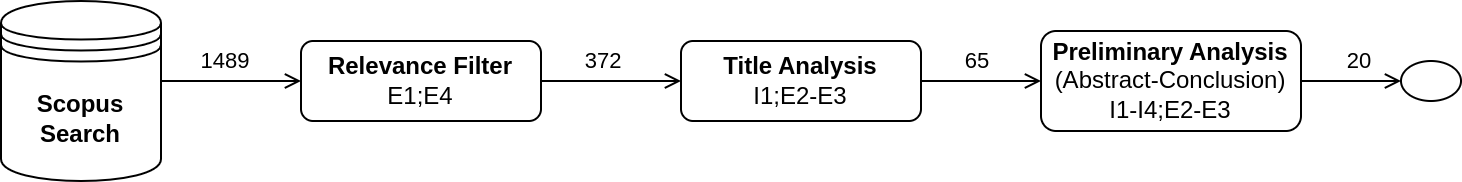
\includegraphics[width=\textwidth]{figures/slr_pipeline.png}
\caption{Systematic Literature Review Pipeline}
\label{fig:slr_pipeline}
\end{figure}




\section{Results}\label{sec:stoa_results}

\begin{description}
    \item[MAD-GAN \cite{li.etal_MADGANMultivariateAnomaly_2019}] is an architecture intended for anomaly detection in multivariate data with spatio-temporal correlations. The generator and the discriminator are composed of Long-Short-Term Recurrent Neural Networks (LSTM-RNN). As is usual in other GANs, the generator creates fake samples from a vector of latent points and feeds them to the generator, whose goal is to distinguish generated from original samples. However, instead of just using the discriminator to detect abnormal samples in the testing phase, the authors propose employing the generator for the same task. The theory for this is that by generating correct samples, the generator can learn the normal distribution of the dataset. 
    
    During the test phase, the discriminator receives a sample from the test dataset and performs the same classification as in the previous stage. However, the generator will receive a version of the sample mapped to the latent space and be tasked with reconstructing the sample. Next, the reconstruction error is calculated by comparing the reconstructed sample with the original one. This error and the discriminator outputs are used to compute the \textit{Discriminator and Reconstruction Anomaly Score} (DR-Score). A sample is considered abnormal if it has a DR-Score higher than a predefined value $\tau$. 
    
    The developed architecture was compared with five baselines. These include PCA, K-Nearest Neighbours (KNN), Feature Bagging (FB), an Autoeconder (AE), and the \textit{Efficient GAN} (EGAN) \cite{zenati.etal_EfficientGANBasedAnomaly_2018a}. The tests were performed on three intrusion detection datasets. MAD-GAN was able to outperform the other baselines on almost all datasets consistently.
\end{description}

\begin{figure}[htp]
\centering
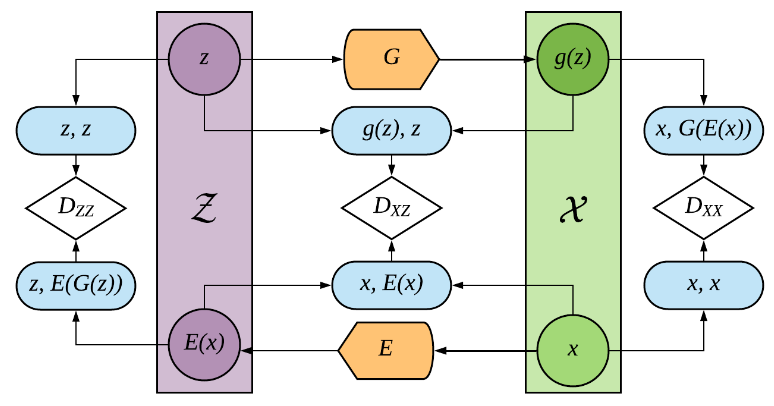
\includegraphics[width=0.8\textwidth]{figures/alad_architecture.png}
\caption[ALAD Architecture]{ALAD Architecture. $D_{xx}$, $D_{xz}$ and $D_{xx}$ are the discriminators (white), $Z$ (purple) and $X$ (green) represent the latent and data spaces, respectively; $G$ and $E$ (orange) are the generator and the encoder, respectively. Reprinted from \cite{zenati.etal_AdversariallyLearnedAnomaly_2018}.}
\label{fig:alad_arch}
\end{figure}

\begin{description}
    \item[ALAD \cite{zenati.etal_AdversariallyLearnedAnomaly_2018}] is a reconstruction-based anomaly detection architecture that employs multiple bi-directional GANs. The proposed method, \textit{Adversarily Learned Anomaly Detection} (ALAD), intends to use both the discriminator and the generator for the task. The ALAD architecture can be seen in Fig. \ref{fig:alad_arch}.
    
    An encoder network $E$ maps data samples $x$ into the latent space $z$ during training. Several additional discriminators are used to achieve cycle consistency (to ensure that the reconstructed samples resemble the original ones) and to provide stability to the model. $D_{xz}$ is an improvement from other similar solutions that solve the saddle-point problem by ensuring cycle consistency, which is not always the case when using encoders. Further entropy regularisation is imposed on both $G$ and $E$ by the discriminators $D_{xx}$ and $D_{zz}$. The latter receives two pairs of latent points and must distinguish the real ($z$, $z$) from the synthesized one ($z$, $E(x)$); the former follows a similar logic but with examples extracted from the dataset. 
    
    The authors propose a new score function for anomaly detection that captures the confidence of $D_{xx}$ when distinguishing real from synthesized pairs. This is because a poor-quality reconstruction would indicate that the generator did not learn how to reconstruct that sample and, consequently, should be considered an anomaly. Finally, the designed model was compared with five standard anomaly detection methods and another GAN for anomaly detection on two anomaly detection datasets. The developed model outperformed the baselines on one of the datasets but could not do so on the other. This was because this dataset had a small number of samples, and ALAD, like other GANs, requires large amounts of training data.
\end{description}

\begin{description}
    \item[USAD \cite{audibert.etal_USADUnSupervisedAnomaly_2020}] is an architecture based on adversarially trained autoencoders for anomaly detection in multivariate time series data, more concretely, logs from IT systems. The authors proposed solving the convergence and mode collapse problems experienced in other GANs. USAD is composed of one encoder $E$ and two decoders $D1$ and $D2$, which in conjunction with the encoder, result in two autoencoders ($AE1$ and $AE2$). $E$ takes data samples as windows $W$ and encodes them to latent space vectors $z$. The function of the decoders is to reconstruct the samples in those windows. 
    
    The autoencoders are trained with normal samples to learn the data distribution during this phase. In the detection stage, both autoencoders are trained adversarially. $AE1$ reconstructs samples from the real dataset and $AE2$ must distinguish examples reconstructed by $AE1$ from the real data. The anomaly score is calculated based on the reconstruction errors obtained on both autoencoders. The proposed model was evaluated along with other unsupervised methods for anomaly detection on intrusion detection datasets. USAD outperformed the other baselines in terms of F1-Score.
\end{description}

\begin{figure}[htp]
\centering
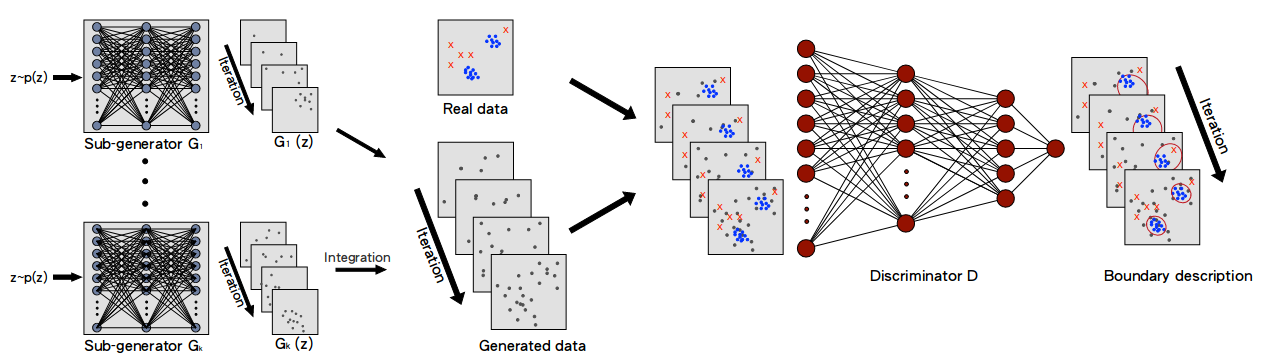
\includegraphics[width=\textwidth]{figures/moogal_arch.png}
\caption[MO-GAAL Architecture]{MO-GAAL Architecture. Each generator $G_i$ to $G_k$ (left) generates outliers for the respective cluster; The discriminator $D$ (right) aims to draw increasingly smaller boundaries around the real data distribution. Taken from \cite{liu.etal_GenerativeAdversarialActive_2020}.}
\label{fig:mo_gaal_arch}
\end{figure}

\begin{description}
    \item[MO-GAAL \cite{liu.etal_GenerativeAdversarialActive_2020}] as the goal of generating informative outliers to overcome the significant class imbalance and lack of correct labels in outlier detection datasets. The authors developed two proximity-based outlier detection methods that do not rely on previous knowledge of the dataset. The first one was given the name of \textit{Single-objective Generative Adversarial Active Learning} (SO-GAAL). Like other GANs, it plays the same mini-max game between the generator $G$ and the discriminator $D$. However, the objective for $G$ is to produce outliers that occur inside or close to the real data. Similarly, the goal of $D$ is to create a division boundary that separates the real data from potential outliers. $G$ gradually learns the generating mechanism and synthesizes an increasing number of potential outliers, and $D$ gets better at creating the divisions that enclose the real data. The point of generating outliers is to create a reasonable reference distribution for the real data. 
    
    Despite providing good results, the first model proved to be very unstable due to the problem of mode collapse. At some point, after a good amount of iterations, the precision of the model would greatly diminish. To solve this issue, another technique called \textit{Multiple-objective Generative Active Learning} (MO-GAAL) was designed. A general workflow of the architecture can be seen in Fig. \ref{fig:mo_gaal_arch}. The authors proposed generating outliers for specific real data subsets using a generator for each cluster in the dataset (which requires cluster identification). This solved the mode collapse problem on the first model and stabilized the performance.  
    
    Both architectures were tested on fourteen datasets and ten other baseline outlier detection methods. Despite other methods performing better in specific datasets, MO-GAAL proved to be more reliable even on non-cluster datasets.
\end{description}

\begin{figure}[htp]
\centering
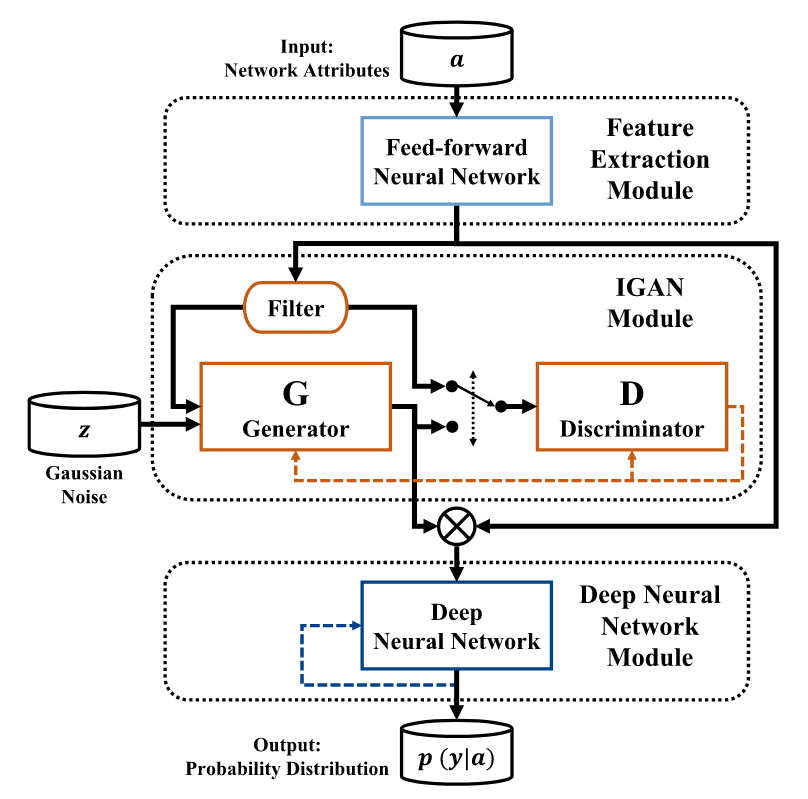
\includegraphics[scale=0.5]{figures/igan_ids_arch.png}
\caption[IGAN-IDS Architecture]{Full IGAN-IDS architecture. Taken from \cite{huang.etal_IGAN_2020}.}
\label{fig:igan_ids}
\end{figure}


\begin{description}
    \item[IGAN-IDS \cite{huang.etal_IGAN_2020}] or \textit{Imbalanced Generative Network} was designed to cope with class imbalance problems that other outlier methods for intrusion detection suffer from. IGAN, which can be seen in Fig. \ref{fig:igan_ids} (middle module) is composed of an imbalanced data filter, Generator $G$, and a Discriminator $D$. Each sample, $s=(x,y)$, is a vector containing the values and the class labels. The imbalanced filter takes only samples from the minority classes, denoted as $s'=(x', y')$. It calculates the generating factor $k$ for each class (ratio of samples that should be generated for each minority class).  $G$ receives a set of latent points $z$ and the class label $y'$ and outputs a vector with a generated value $G(z,y')$ from the class label that it received. This vector is then passed to the discriminator, which aims to distinguish synthesized feature vectors from the ones extracted from the dataset. In the training process, $G$ and $D$ are trained alternatively. First, $D$ is fed only real samples while $G$ is fixed, and in the next iteration, $G$ is optimized, and $D$ is fixed. 
    
    With the problem of class imbalance dealt with, the authors set out to perform intrusion detection with IGAN-IDS (Fig. \ref{fig:igan_ids}). The feature extraction module (top) embeds discrete data into one-hot encoded vectors and discretizes continuous variables, which are encoded. All values are concatenated and fed to IGAN, which generates samples for the imbalanced classes. Finally, a DNN (bottom module) is used for outlier detection. In the training stage, it receives both synthesized and real data and, during the testing phase, calculates the distributed probabilities for each inclusion class of each sample. The proposed solution was tested with several other class-balancing techniques on three standard intrusion detection datasets. It outperformed every method in precision, accuracy, recall and AUC score.
\end{description}


\begin{description}
    \item[Jiang et al. (2019) \cite{jiang.etal_GANBasedAnomalyDetection_2019}] propose a conditional GAN architecture to detect anomalies in univariate Industrial Time Series Data. The model is trained with only normal samples. The dimensionality of the original data was reduced by employing a feature extractor. The generator consists of two encoders $G_e$ and $G_{e'}$ and an intermediate decoder $G_d$. The first encoder maps real samples into the latent space $z$ while the decoder $G_d$ is tasked with reconstructing the encoded sample back to the real data space. 
    
    During training, the GAN is only tasked with reconstructing normal data samples so that both components learn the normal distribution of the dataset. Two loss functions are defined for the generator, the \textit{Apparent loss} and the \textit{Latent loss}. The first measures the distance between the original and synthesized samples, and the other measures the distance between the latent vectors $z$ and $z´$ encoded by $G_e$ and $G_{e'}$, respectively. The loss function of the discriminator compares the feature vector from the actual sample $f(x)$ with the synthesized one $f(G(x))$. The anomaly score is defined as the sum of the two losses. 

In the testing phase, two rolling bearing datasets were used. The authors fine-tunned the models by adjusting the hyper-parameters of the network. A significant difference in anomaly score $A(x)$ was observed for faulty parts in the dataset, which proved the efficacy of the designed model. A comparison was also performed with the state-of-the-art BiGAN \cite{donahue.etal_AdversarialFeatureLearning_2017}, which showed that the developed GAN was more reliable on datasets with differing sizes.
\end{description}

\begin{description}
    \item[TadGAN \cite{geiger.etal_TadGANTimeSeries_2020}] aims to solve the problem of scalability and portability in state-of-the-art unsupervised methods for anomaly detection. Its goal is to detect anomalies in time series datasets. The authors used LSMT Recurrent Neural networks for both the generator and the critic. Two types of anomalies are identified single point (abnormal data point) and collective (sequence of abnormal data points) anomalies. 
    
    The proposed architecture is a reconstruction-based anomaly detector with a generator $G$ which receives encoded samples in the form of latent points $z$ and reconstructs them back to the original sample distribution; an encoder that takes samples in the normal distribution and encodes them into latent point vectors; and two critics, one to distinguish real data points from synthesized ones ($C_x$) and the other ($C_z$) to evaluate between the distribution of real $z$ and the ones that were encoded by $E$ ($E(x)$). To cope with the mode collapse problem, common in most GANs, the authors adopt the Wasserstein loss function (for critics) and a cycle consistency loss function (for the generator and encoder). For the reconstruction errors, the point-wise difference (distance between the real and synthesized point)  and area difference (distance between "windows" of the same area in the real and synthesized data) were defined. Furthermore, the authors also chose a \textit{Dynamic Time Warp} (DWT) measure, which, similarly to area difference, can identify minor differences over long periods but can also handle time shift issues. 
    
    Two methods of combining the critic outputs with the reconstruction errors were devised. For the first, a weighted sum of the reconstruction error and the critic output is done; in the other method, both values are directly multiplied. Several baselines are chosen to compare with the developed model in the testing phase. TadGAN and the baselines were tested on eleven datasets for anomaly detection (two of which were from NASA). The developed network outperformed every other baseline on six of the eleven datasets (based on the F1-score). Despite this, the mean, standard deviation and average of the F1-score in all datasets showed that TadGAN was more reliable than the other methods. Finally, the authors defined ten iterations of TadGAN, each with a different anomaly score with either one reconstruction function, one critic output or a combination of the two. The worst result was with the anomaly function consisting only of the critic output, and the best was the one in which the critic score and DWT were multiplied.
\end{description}

\begin{description}
    \item[adVAE \cite{wang.etal_AdVAESelfadversarialVariational_2020}] employs a Variational Autoencoder (VAE) for anomaly detection. The authors propose an encoder $E$ that encodes real samples into random point vectors $z$, fed to a generator $G$ that is then tasked with synthesizing examples close to the real distribution of the dataset. Competition is introduced in the form of a Gaussian transformer $T$ that receives the encoded vectors from $E$ and is tasked to generate latent vectors $z_T$ with a similar distribution to $z$ (outliers). $G$ is tasked with generating as different as possible examples from both similar latent vectors. Finally, the examples from $G$ are encoded again by $E$, and the resulting distributions are compared with the original ones. To make the equilibrium of these three models feasible, the authors freeze the gradients of $E$ in the first training phase to only train the $G$ and $T$. This way, $T$ will generate abnormal latent variables close to the real distribution, and $G$ will be able to distinguish them using reconstruction errors. 
    
    In the second phase, both $G$ and $T$ have their gradients frozen, and the encoder is trained to encode the inputs as close as possible to the prior distribution (only if the inputs are from the dataset and do not result from Gaussian variables generated by $T$). In the testing phase, the trained encoder and generator are used to detect anomalies by calculating the reconstruction error of the input samples. The solution was evaluated on tabular anomaly detection datasets and several other state-of-the-art outlier detection methods. Furthermore, several ablation models from adVAE were derived by removing the discriminative factors of either the generator or the encoder. The results showed that adVAE and its variations outperformed most baselines on the chosen datasets regarding precision and AUC score. 
\end{description}

\begin{description}
    \item[Blance et al. (2019) \cite{blance.etal_AdversariallytrainedAutoencodersRobust_2019}] propose using adversarially trained autoencoders as a way of improving the separation between background from the signal in synthesized high-energy collision events. The authors train an NN that can distinguish signal events from the background and intentionally smear the background data in distinct directions. With this, they prove that the classifier's performance is highly dependent on the smearing of the background samples.

    An adversary is used to try and remove the dependence of the classifier on the smearing of samples. Both are forced into a zero-sum game in which the classifier must learn how to make predictions without using any information from smearing and tries to make it as hard as possible for the adversary to discriminate the background samples. The classifier receives samples from the dataset and sends its outputs to the adversary, which tries to determine the background class based on the outputs. The results showed that this method significantly reduced the dependence of the classifier on the smearing of background samples.

    In addition, the authors propose another method in which they use an autoencoder alongside an adversary. The function of the autoencoder is to reconstruct only background samples, and the adversary is tasked with identifying them. As the autoencoder only learns the distribution of background events, it will not be able to reconstruct signal events as well (i.e. signal events will be considered outliers). The adversary takes as input the loss of the AE and tries to determine the background smear class. The results show that the method could remove the dependence between the autoencoder classification and the smear direction of the background samples. Despite this, this architecture proved less effective than the previous one.
\end{description}

\begin{description}
    \item[FGPAA \cite{wu.etal_FaultAttentionGenerativeProbabilistic_2020}] is an adversarially trained autoencoder that aims to monitor the conditions of roll-bearings by analyzing the vibration signals. The model consists of four components, a discriminator $D$, a generative discriminator $GD$, an encoder $E$ and a Low-dimension discriminator $LD$. $E$ takes one signal at a time and encodes it into the low-dimension manifold (latent space) $z$. $LD$ discriminates if the output of the encoder follows the same distribution as the latent space $z$. The latent points vector $z$ is passed to the encoder that works as a generator by synthesizing high-dimension signals from the low manifold distribution. The generative discriminator, $GD$,  tries to distinguish reconstructed signals from those originating from the dataset.

    The anomaly score is calculated for each sample by comparing the distributions of the generated low-dimension manifold and the reconstructed sample with the distributions from the actual dataset. This score is then used during detection to identify signal data faults. The proposed solution was tested on three roll-bearing datasets alongside well-known ML anomaly detection methods. FGPAA outperformed all in terms of F1-score, but they displayed a higher execution time than the rest.
\end{description}

\begin{description}
    \item[FGAN \cite{ngo.etal_FenceGANBetter_2019}] is an architecture close to original GANs but with a modified loss function more suited for anomaly detection. The authors propose adapting the model's objective so that the generated samples lie close to the boundaries of the real data distribution instead of overlapping it. The objective is to generate data around low data density regions $\delta X$ around the real dataset.

    The authors use the discriminator score to identify the domain of $\delta X$ and then estimate it with the generator. At the end of the training phase, the synthesized points must enclose the entirety of the data. This goal is achieved by replacing the typical loss of the generator with the \textit{Generator Encirclement Loss}, which penalizes points generated inside or far away from the real distribution. \textit{Generator Dispersion Loss} is also introduced to guarantee that the generated points enclose the whole distribution and not just a single area (similar to mode collapse in other methods). It maximizes the distance between points by penalizing the generator if the synthesized points are too close to each other. The resulting loss function is a weighted sum of the two proposed ones. Similar to the generator, the loss function of the discriminator is also modified to prioritize classifying real data correctly by reducing the second term of the original discriminator function (refer to equation \ref{eq:gan_min_max}).

    To evaluate the developed mode, the authors tested its performance on a synthesized 2D dataset. Next, the proposed solution was tested on image and tabular datasets and other state-of-the-art models. FGAN outperformed all baselines for anomaly detection on both types of datasets.
\end{description}

\begin{description}
    \item[MENSA \cite{siniosoglou.etal_UnifiedDeepLearning_2021}] is an autoencoder-based GAN architecture used to detect intrusions on next-generation Electrical Grids (also known as Smart Grids). Furthermore, the proposed model can also detect and classify different classes of cyberattacks that often occur on the TCP (Transport Communication Protocol) and the DNP3 (Distributed Network Protocol 3) protocols.

    The architecture consists of a Generator-Encoder and a Discriminator-Encoder. The first receives input noise samples and inflates them to produce samples that resemble the desired data to learn the normal distribution. The Discriminator-Encoder then compresses the synthesized samples into a single point that indicates if the sample is from the real dataset or is a fake. For the detection phase, the Latent Model is derived from the initial layers of the discriminator. The generator, having learned the normal distribution of the data, tries to reconstruct samples from the real dataset. These are then passed to the Latent Model that calculates the Adversarial Loss score by comparing the real sample with the reconstructed one. Note that the generator will fail to reconstruct abnormal samples, as they were not a part of the training process.

    The classification model is derived from the previous architecture, in which the Discriminator-Encoder also learns to classify the attack class of a given sample. The generator learns to generate samples based on the class labels conditionally. Similar to the previous implementation, the discriminator receives the synthesized samples and identifies them as real or fake, but this time, it also tries to determine the class label.  

    The proposed solution was tested on real Smart Grid datasets and several other intrusion detection methods. The Accuracy, True-Positive and False-Positive rates and F1-Score were calculated for each solution. MENSA outperformed other methods on all datasets except for one.
\end{description}

% rever
% \begin{description}
%     \item[Sun et al. (2019) \cite{sun.etal_TimeSeriesAnomaly_2019}] propose applying a GAN to the detection of anomalies in vehicles. The data used for this purpose was extracted over three years with sensors placed inside several buses. With this, the authors set out to develop a model that could detect anomalies in the buses' components within a reasonable time period. For this solution, only the engine stall failure category was used.

%     The model's architecture consists of a generator with a linear layer network and a discriminator based on CNNs. The latter was chosen for the capacity of feature extraction and the ability of CNNs to handle spatial data. The generator learns the normal dataset distribution while the discriminator distinguishes real sensor measures from fake ones. The concept of dynamic threshold is introduced for the anomaly detection score. When the discriminator receives an abnormal example from the actual dataset, it is forced to classify the fake sample from the generator as real. This misclassification is then to determine that the actual sample from the dataset is an anomaly.
    
%     The results proved that the discriminator was able to detect anomalies confidently.
% \end{description}

\begin{figure}[ht]
\centering
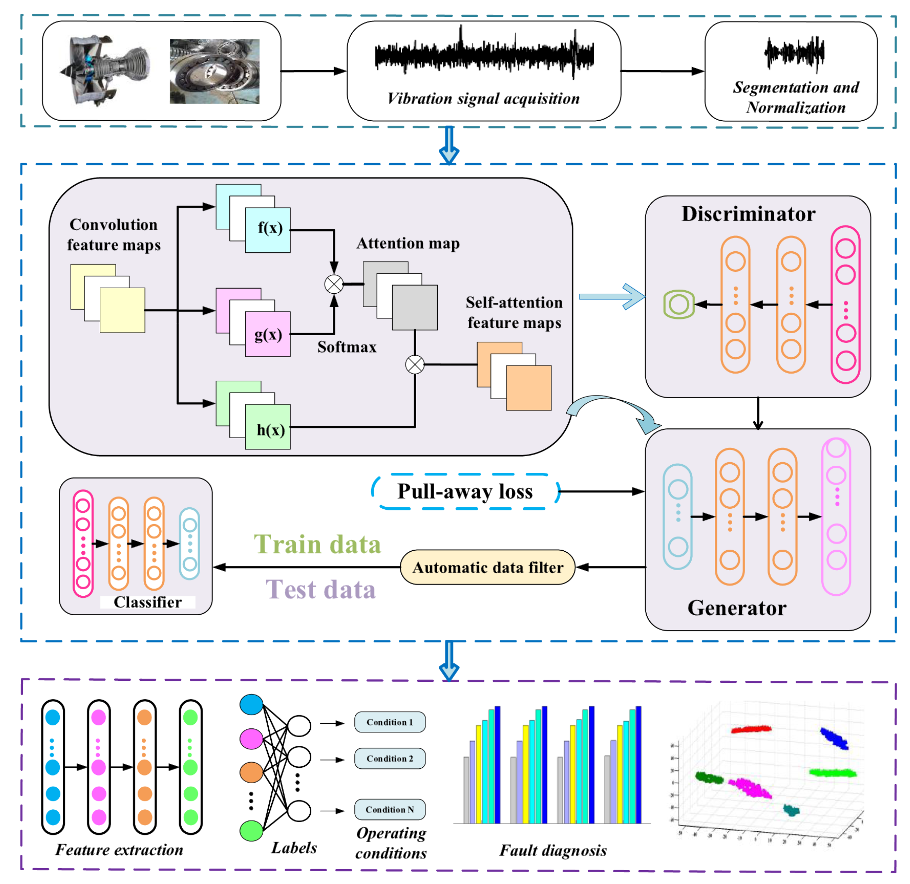
\includegraphics[scale=0.4]{figures/liu.etal_2022.png}
\caption[Roll bearing anomaly methodology]{Methodology for anomaly detection in roll bearing datasets. Taken from \cite{liu.etal_DataSynthesisUsing_2022}.}
\label{fig:liu.etal_2022}
\end{figure}

\begin{description}
    \item[Liu et al. (2022) \cite{liu.etal_DataSynthesisUsing_2022}] propose a deep feature enhanced generative adversarial network to improve fault detection performance in roll bearing imbalanced datasets. New and preexisting methods are introduced to solve mode-collapse during training and enhance the feature learning of the network, which aim to increase the overall detection performance of the architecture. The adopted methodology can be seen in Fig. \ref{fig:liu.etal_2022}.

    A new loss function is designed for the generator with a \textit{pull-away} term. It measures the distance between the generated samples inside a given batch and penalizes the generator if the batch's samples are too similar. As a consequence, this solves the mode-collapse problem during the training phase. A self-attention model is introduced to the discriminator and the generator so they can learn the features of the original vibration signals more deeply. The self-attention feature maps capture local details and global information in every layer of the network.

    During training, the generator synthesizes signals from random noise fed to the discriminator along with an actual signal. The discriminator must then distinguish which one is real and which one is fake. With the proposed mechanisms, the generator must synthesize samples as far as possible to each other to confuse the discriminator. The training phase stops when three criteria are met. These are defined by the \textit{automatic data filter}, which evaluates the accuracy and diversity of the generated samples based on discriminator probability, Kullback-Leibler (KL) divergence and maximum mean discrepancy.  When these criteria surpass a predefined threshold, the training phase is concluded. The fault detection phase uses a classifier trained on the generated data.  

    The quality of synthesised signals was compared with other standard generative models using KL divergence and maximum mean discrepancy of the \textit{automatic data filter}. The proposed method surpassed the others in these metrics. Next, three experiments were set up to evaluate the detection quality of the proposed method. In each experiment, three classifier models were used. In the first, the classifiers learned to detect anomalies from the original signals dataset. In the next, a WGAN-GP architecture was used to generate a more balanced signals dataset. Finally, the three classifiers were trained on data synthesized by the proposed method in the last experiment. This methodology was performed on laboratory and locomotive roll-bearing datasets. Every model trained on the generated data (for both datasets) from the designed solution outperformed the models from the other experiments.

    
\end{description}

% Incomplete
% \begin{description}
%     \item[OD-GAN \cite{oh.etal_OGAN_2019}] is a conditional GAN that uses oversampling to generate samples of the minority class while removing outliers from the majority class. Both the generator $G$ and the discriminator $D$ have the same goals as on the original GAN architecture proposed by Goodfellow et al. \cite{goodfellow.etal_GenerativeAdversarialNets_}. The difference is that in OC-GAN, during training, only the samples of the minority class are considered. The authors define Dissimilarity with the Minority Class score ($DWM_i$), which measures the distance between a sample and the data distribution for the minority class. Samples much further away from the normal distribution have a larger $DWM_i$ and are considered outliers. To detect anomalies, the majority class samples are ordered in accordance with the distance to the minority class. Normal samples lie close to the minority distribution while outliers are recorded when there is a rapid variation in the $DWM_i$ distance.
    
    
%     Data samples that are too close or far away from the minority class are classified as outliers of the majority.
% \end{description}

\begin{description}
    \item[DOPING \cite{lim.etal_DOPINGGenerativeData_2018}] is an adversarial autoencoder that aims to improve the performance of unsupervised anomaly detection by oversampling \textit{infrequent normal samples}. With this, the authors intend to reduce the number of false positives that usually occur on datasets with normal samples close to the classification boundary (close to but not anomalies). 

    In the training phase, the autoencoder receives samples from the entire dataset distribution. The latent vectors generated by the encoder, $E$, from the data samples, $X$, are saved for the next stage, in which only the latent variables $Z$ at the tail-end distribution of the normal data are sampled into a pool of $Z_{edge}$. From this pool, $z_{edge}$ variables are then sampled randomly and interpolated to generate new latent vectors $z_{new}$. In the next stage, de decoder $D$ synthesizes minority samples from the $z_{new}$ latent vectors. Later the synthesized examples can be used in conjunction with the original ones for anomaly detection.

    An isolation forest anomaly detector was used to evaluate the effects of the oversampling method on the detection performance. The authors used three synthesized cluster datasets with outliers, the popular MNIST image dataset, and four real medical record datasets. The results showed that the outlier detection method in conjunction with DOPING achieved better results than the baseline (detection without DOPING). 
\end{description}

\begin{description}
    \item[Bot-GAN \cite{yin.etal_EnhancingFrameworkBotnet_2018}] aims to improve the detection performance of botnets in network-flow data. The architecture is similar to the one from vanilla GAN. However, the authors chose a botnet detection model as a discriminator. Like vanilla GAN, it receives examples from the training dataset and synthesizes ones from the generator. The main difference is that the discriminator classifies each sample as normal (from the training dataset), an anomaly or fake (either synthesized or from the dataset). The generator's objective is to synthesize more samples similar to the ones in the dataset to assist with the training of the detector.

    To test the proposed approach, choose a botnet dataset and perform some preprocessing to normalize the formats of the entries and map the features into vectors. The resulting feature maps are then scaled so that each value falls between [-1,1]. The model was evaluated on precision, accuracy, false positive rate, recall and F1-Score. The results show that it is possible to improve the performance of the classification model by enhancing its training with GANs.
\end{description}

\begin{description}
    \item[Yuan et al. (2020) \cite{yuan.etal_OutageDetectionPartially_2020}] propose employing GANs to learn the normal conditions of smart meter operations to detect power outages in electrical grid zones. In addition, the authors propose circumventing the problems of other models applied to this problem, which are the assumption that every network node is directly observable. The distribution network is subdivided into zones determined by two neighbouring observable nodes (nodes in which the voltage and demand). Each zone has its designated GAN, which learns the time-series data collected by the two nodes. Any deviation from each node's normal measured data distribution will be considered an anomaly.

    The architecture is very similar to the one on vanilla GAN \cite{goodfellow.etal_GenerativeAdversarialNets_}. The generator's objective is to synthesize Time-Windows (frames with recorded sequential events) with events similar to the ones from the assigned zone. Similarly, the discriminator must distinguish between real and fake Time-Windows. At the end of the training phase, both components captured the normality of the data for the given zone.

    In the detection phase, both generator and the discriminator are used. Time-Windows with actual recorded events are fed to the latter, which calculates the Discrimination Loss. Additionally, an inverted mapping of the Time-Window to the latent space is given to the generator, which is tasked with reconstructing it. The weighted sum of the reconstruction error and discriminator loss is used to calculate the Anomaly Score.

    The solution is evaluated on data collected over three years by smart meters on a complex power distribution network. The results proved that the proposed approach could reliably detect power outages in real distribution networks. Finally, numerical comparisons are performed to compare the developed method with a preexisting SMV model to detect power outages. The authors conclude that the developed GAN can achieve better results (in terms of accuracy) with a significantly reduced amount of data.
\end{description}

\begin{description}
    \item[AMBi-GAN \cite{kong.etal_IntegratedGenerativeModel_2023}] is bidirectional LSTM GAN for anomaly detection in industrial multidimensional time-series data. Unlike univariate time series, multivariate time series consists of multiple measurements in a given time step. The authors propose solving the difficulties of other methods in extracting temporal information, feature extraction and lack of large amounts of labelled data.

    The architecture consists of a discriminator and a generator using the same bidirectional LSTM network (AMBi-LSTM). An attention mechanism is also proposed to learn the importance of each time-series element. It calculates a given sample's weight to determine how much it should affect the parameters in the network.

    In the training phase, each sample is extracted using a sliding window that subdivides the whole dataset into equal-length subsequences (each with multiple values for a given time). The generator's goal is to generate windows with the same distribution as the original ones. The discriminator receives real and false samples and must distinguish between them.

    When both components have reached an equilibrium, anomaly detection can be performed. Random samples are extracted from the testing dataset and fed directly to the discriminator. At the same time, the samples suffer from inverted mapping into the latent space, so they can be given to the generator, whose goal is to reconstruct them as well as possible. Next, the \textit{Discriminator Score} is calculated by combining the loss from the discriminator and the reconstruction error from the generator. 

    AMBi-GAN and the other two baselines were evaluated on precision, recall and F1-score on three time-series datasets. The proposed solution outperformed the other baselines on every metric. In addition, several variations of AMBi-GAN were developed, from changing the number of hidden layers of AMBi-LSTM to assess which one performed better on the chosen datasets.
\end{description}

\begin{description}
    \item[TAnoGAN \cite{bashar.nayak_TAnoGANTimeSeries_2020}] was designed to detect anomalies in industrial time-series data with a small number of samples. The model consists of a generator $G$ and a discriminator $D$, with both architectures based on LSTM networks. In the training phase, $G$ learns to generate realistic time-series sequences from a latent space distribution, and $D$ distinguishes fake samples from real ones. The samples consist of small time series sequences extracted from the dataset with a sliding window method. 
    
    In the detection phase, real-time-series samples are mapped to the latent space and then reconstructed by $G$. Anomaly detection is done by evaluating the reconstruction error of the synthesized sample with the original one. Mapping from the original sample to the latent space is done iteratively. First, a random sample $z^i$ from the latent space $z$ is chosen and fed to $G$, which generates a fake sample. The resulting fake data $G(z^i)$ is compared to the original sample $x$ with a point-wise dissimilarity measure $L_R$. Next, the parameters of $z^i$ are updated and thus, in the next iteration, the reconstructed sample will more closely resemble the authentic one. This process is repeated $\Lambda$ times (a predefined parameter). At the end of the inverse mapping, the final $z^i$ is compared to the original sample, and the anomaly score is obtained with the weighted sum of $L_R$ and the discriminator loss $L_D$.

    To deal with the small number of samples in the datasets, the authors varied the number of hidden layers in each architecture. It was observed that discriminators with many hidden layers easily overfitted the data. In contrast, generators with small numbers of hidden layers failed to synthesize realist time series sequences. 

    The solution is evaluated on a large number of time-series datasets along with other unsupervised state-of-the-art anomaly detection methods. The performance (measure in accuracy, recall, F1-score, AUC, and Cohen Kappa Score) demonstrates that TAnoGAN is more suited than other models to detect anomalies in small time-series datasets.
\end{description}

\begin{description}
    \item[MinLGAN \cite{wang.etal_AnomalyDetectionMinimum_2018}] aims to detect outliers by generating both normal and abnormal samples during the training phase. The authors employ minimum likelihood regularisation to the generator, $G$, to produce more abnormal samples and prevent them from converging to the normal distribution of the data. This solution ensures that the performance of the discriminator, $D$, does not deteriorate in the final phases of training as it receives samples from the generator that are increasingly closer to the real distribution of data. The regularization is done by adapting the loss function of the generator with a KL divergence measure. It penalizes the generator when the produced samples are distributed close to the dataset and, thus, prevents the convergence of $G$ with the original data distribution. 

    To deal with the instability of the discriminator in the early phases of training resulting from the data's randomness, the authors propose \textit{Ensemble learning}. Two ensemble methods are presented, which are bagging and boosting. The latter consists of a set of models trained from random subsamples of the training dataset. In contrast, the models are obtained in the former by emphasizing training samples that other models misclassified. The authors independently trained a set of $D$ models in line with this. The outputs of each discriminator (before sigmoid activation) are combined into a single value in two different score functions for anomaly detection (one is scaled to account for the minimum and maximum ranges of the outputs).

    In the experimentation phase, three GANs were created. One baseline MinLGAN and two other models with ensemble learning and the score functions that were defined. All of them were trained along with five other unsupervised anomaly detection approaches on an image and several tabular datasets. Despite providing good results in all datasets, the authors pointed to the difficulty felt in the training phase due to the complexity of the proposed approach.
\end{description}

\begin{description}
    \item[ATTAIN \cite{xu.etal_DigitalTwinbasedAnomaly_2021}] is an architecture that makes use of GANs to detect anomalies in cyber-physical systems (CPS). Unlike other methods, ATTAIN can learn data distribution at runtime without needing static data. This allows it to adapt to previously unseen novel attacks continuously. 

    The solution consists of a Digital Twin Model, a digital replica of a real system, and a Digital Twin Capability; the GAN used for anomaly detection. The first model is built with historical and real-time measurements from sensors and actuators, while the detector only learns from real-time data. The generator's objective is to produce samples from the latent distribution into the original data distribution. The function of the discriminator is to distinguish between normal, and attack samples that come either from real-time or are synthesized by the generator. Therefore, the output of the discriminator consists of four categories. 

    The generator, $G$, is composed of an input layer which encodes discrete values into one-hot vectors; a Graph Convolutional Layer (GCN) that is tasked with learning the independent relationships between sensors and actuators; a pooling layer which collapses the outputs of the previous layers; and an LSTM layer with the function of retaining the temporal features of the data. The discriminator receives both real and generated samples, which are concatenated and suffer a linear transformation. Next, the resulting vector is passed through a \textit{tahn} activation function before being passed to the next layer. The following step calculates a ground truth label for the received fake sample. It is first given to the Digital Twin Model that predicts its state, and later, the hamming distance $d$ between the predicted and real state is obtained to help in the labelling process. The discriminator determines if the sample is real or fake. In the case of the latter the $d$ measure from the previous step is compared to determine if the example is a regular or attack adversarial sample. The loss between the ground truth and the likelihood (obtained by softmax of the output of $D$) is calculated in the final layer.

    The designed model was tested with two other baselines on three intrusion detection datasets. The performance metrics were outlier precision, recall and F1-score. A comparison of all the results shows that using the digital twin model to guide the training of the GAN improved the overall outlier detection capability of the model compared to the other solutions. However, the authors recognize the possible threats to validity as they could not test the solution on a real CPS system. 
\end{description}


\section{Analysis}\label{sec:res_analysis}
In Table \ref{tab:slr_results}, a brief analysis of the SLR results will be carried out to study the effectiveness of the chosen methodology. Aside from the paper name and year, four other categories were identified to compare the evaluated solutions:

\begin{itemize}
    \item \textbf{Training Objective:} this category aims to describe the training approach for a given model. With this, the goal is to compare models that fit the normal data distribution during the training phase and other alternatives. This allows for a straightforward summary of the training approaches that can be adopted to solve the proposed problem.

    \item \textbf{Anomaly Detection:} in this group, the goal is to identify several of the approaches that can be used to detect anomalies. These methods can be relative to calculating an anomaly score or, in some cases, using classifiers to achieve this goal. The possible values for this category include Reconstruction errors, Discriminator Loss (D loss) and Classifiers.

    \item \textbf{Architecture:} this class aims to analyse the different types of architectures defined in each of the papers. These can be "Normal" in the case they use the vanilla composition of GANs;  "Mixed" when other components like encoders, $E$, classifiers, $C$, feature extractors (FE) and Self-attention devices (SA)\footnote{Module used during the training phase to make the discriminator and generator learn the data features more thoroughly.} are used; and autoencoders (AE).

    \item \textbf{Application:} this last category describes the specific problem that each of the designed models tries to solve (i.e. the scenario to which they are applied). Some models have no direct application and can be used in many types of problems, and because of this, they have no assigned application (N/A)
\end{itemize}



\bgroup
\def\arraystretch{1.5}
\begin{table}
\caption{List of reviewed papers.}
\label{tab:slr_results}
 \begin{adjustwidth}{-1.8cm}{}
\resizebox{0.9\textwidth}{!}{\begin{minipage}{\textwidth}
\centering
\begin{tabular}{cccccc} 
\toprule
Paper         & Year & Training Objective                                                             & Anomaly Detection         & Architecture   & Application                                                        \\ 
\hline
MAD-GAN  \cite{li.etal_MADGANMultivariateAnomaly_2019}     & 2019 & Normal                                                                         & Reconstruction + D loss           & Normal         & Time Series                                                        \\ 
\hline
ALAD \cite{zenati.etal_AdversariallyLearnedAnomaly_2018}         & 2018 & Normal                                                                         & Reconstruction            & Mixed (E)      & N/A                                                                \\ 
\hline
USAD \cite{audibert.etal_USADUnSupervisedAnomaly_2020}         & 2020 & Normal                                                                         & Reconstruction            & AE             & N/A                                                                \\ 
\hline
MO-GAAL \cite{liu.etal_GenerativeAdversarialActive_2020}      & 2020 & \begin{tabular}[c]{@{}c@{}}Outlier Generation \\Division Boundary\end{tabular} & Classifier                & Mixed (C)      & N/A                                                                \\ 
\hline
IGAN-IDS \cite{huang.etal_IGAN_2020}     & 2020 & Outlier Oversampling                                                           & Classifier                & Mixed (FE + C) & Intrusion Detection                                                \\ 
\hline
Jiang et al. \cite{jiang.etal_GANBasedAnomalyDetection_2019}  & 2019 & Normal                                                                         & Reconstruction            & AE             & Time Series                                                        \\ 
\hline
TadGAN \cite{geiger.etal_TadGANTimeSeries_2020}       & 2020 & Normal                                                                         & Reconstruction~ + D loss  & Mixed (E)      & Time Series                                                        \\ 
\hline
adVAE \cite{wang.etal_AdVAESelfadversarialVariational_2020}        & 2020 & Normal                                                                         & Reconstruction            & AE             & N/A                                                                \\ 
\hline
Blance et al. \cite{blance.etal_AdversariallytrainedAutoencodersRobust_2019} & 2019 & Outlier Oversampling                                                           & Classifier                & AE             & High Energy Physics                                                \\ 
\hline
FGPAA \cite{wu.etal_FaultAttentionGenerativeProbabilistic_2020}        & 2020 & Normal                                                                         & Reconstruction            & Mixed (AE)     & Roll Bearing Fault                                                 \\ 
\hline
FGAN \cite{ngo.etal_FenceGANBetter_2019}         & 2019 & \begin{tabular}[c]{@{}c@{}}Normal\\Division Boundary\end{tabular}              & D loss (adapted) & Normal         & N/A                                                                \\ 
\hline
MENSA \cite{siniosoglou.etal_UnifiedDeepLearning_2021}        & 2021 & Normal                                                                         & D (initial layers)        & AE             & Intrusion Detection                                                \\ 
\hline
Liu et al. \cite{liu.etal_DataSynthesisUsing_2022}   & 2022 & Normal                                                                         & Classifier                & Mixed (C + SA) & Roll Bearing Fault                                                 \\ 
\hline
DOPING \cite{lim.etal_DOPINGGenerativeData_2018}       & 2018 & Minority Oversampling                                                          & Classifier/Model          & AE             & \begin{tabular}[c]{@{}c@{}}Performance \\Improvement\end{tabular}  \\ 
\hline
Bot-GAN \cite{yin.etal_EnhancingFrameworkBotnet_2018}      & 2018 & Normal                                                                         & Classifier (D)            & Normal         & Bot Detection                                                      \\ 
\hline
Yuan et al. \cite{yuan.etal_OutageDetectionPartially_2020}   & 2020 & Normal                                                                         & Reconstruction            & Normal         & \begin{tabular}[c]{@{}c@{}}Power Outage \\ Detection\end{tabular}  \\ 
\hline
AMBi-GAN \cite{kong.etal_IntegratedGenerativeModel_2023}      & 2021 & Normal                                                                         & Reconstruction + D loss   & Normal         & Industrial Time Series                                             \\ 
\hline
TAnoGAN \cite{bashar.nayak_TAnoGANTimeSeries_2020}      & 2020 & Normal                                                                         & Reconstruction            & Normal         & Time Series                                                        \\ 
\hline
MinLGAN \cite{wang.etal_AnomalyDetectionMinimum_2018}      & 2018 & All Data                                                                       & D                         & Normal         & N/A                                                                \\ 
\hline
ATTAIN \cite{xu.etal_DigitalTwinbasedAnomaly_2021}       & 2021 & Normal                                                                         & D Loss                      & Normal         & Cyber-physical Systems                                             \\
\bottomrule
\end{tabular}
\end{minipage}}
\end{adjustwidth}
\end{table}
\egroup

% \begin{table}[htbp]
% \caption{List of reviewed papers.}
% \label{tab:slr_results}
%  \begin{adjustwidth}{0.5cm}{}
% \resizebox{0.8\textwidth}{!}{\begin{minipage}{\textwidth}
% \begin{tabular}{cccccc} 
% \hline
% Paper                         & Year                      & Training Objective                                                                  & Anomaly Detection                                                    & Architecture                                                    & Application                                                             \\ 
% \hline
% MAD-GAN                       & 2019                      & normal distribution                                                                 & G loss + D loss                                                      & Normal                                                          & Time series                                                             \\ 
% \hline
% ALAD                          & 2018                      & normal distribution                                                                 & Reconstruction                                                       & Mixed (E)                                                       & N/A                                                                     \\ 
% \hline
% USAD                          & 2020                      & normal distriution                                                                  & Reconstruction                                                       & Autoencoder                                                     & N/A                                                                     \\ 
% \hline
% MO-GAAL                       & 2020                      & \begin{tabular}[c]{@{}c@{}}outlier generation\\ division boundary\end{tabular}      & Classifier                                                           & Mixed (C)                                                       & N/A                                                                     \\ 
% \hline
% IGAN-IDS                      & 2020                      & outlier oversampling                                                                & Classifier                                                           & Mixed (FE + C)                                                  & Intrusion detection                                                     \\ 
% \hline
% Jiang et al.                  & 2019                      & normal distribution                                                                 & Reconstruction                                                       & Autoencoder                                                     & Time series                                                             \\ 
% \hline
% TadGAN                        & 2020                      & normal distribution                                                                 & \begin{tabular}[c]{@{}c@{}}Reconstruction \\ and D loss\end{tabular} & Mixed (E)                                                       & Time series                                                             \\ 
% \hline
% adVAE                         & 2020                      & normal distribution                                                                 & Reconstruction                                                       & Autoencoder                                                     & N/A                                                                     \\ 
% \hline
% Blance et al.                 & 2019                      & outlier oversampling                                                                & Classifier                                                           & Autoencoder                                                     & High energy physics                                                     \\ 
% \hline
% FGPAA                         & 2020                      & normal distribution                                                                 & Reconstruction                                                       & \begin{tabular}[c]{@{}c@{}}Autoencoder\\ and G + D\end{tabular} & \begin{tabular}[c]{@{}c@{}}Roll bearing\\ fault detection\end{tabular}  \\ 
% \hline
% FGAN                          & 2019                      & \begin{tabular}[c]{@{}c@{}}normal distribution\\ and division boundary\end{tabular} & \begin{tabular}[c]{@{}c@{}}G loss + D loss \\ (adapted)\end{tabular} & Normal                                                          & N/A                                                                     \\ 
% \hline
% MENSA                         & 2021                      & normal distribution                                                                 & D (initial layers)                                                   & Autoencoder                                                     & Intrusion detection                                                     \\ 
% \hline
% Liu et al.                    & 2022                      & normal distribution                                                                 & Classifier                                                           & \begin{tabular}[c]{@{}c@{}}Mixed\\(C +SA)\end{tabular}          & \begin{tabular}[c]{@{}c@{}}Roll bearing\\fault detection\end{tabular}   \\ 
% \hline
% DOPING                        & 2018                      & \begin{tabular}[c]{@{}c@{}}oversampling\\ normal min.\end{tabular}                  & Classifier/Model                                                     & Autencoder                                                      & \begin{tabular}[c]{@{}c@{}}Performance \\ improvement\end{tabular}      \\ 
% \hline
% Bot-GAN                       & 2018                      & normal distribution                                                                 & Classifier (D)                                                       & Normal                                                          & Bot detection                                                           \\ 
% \hline
% Yuan et al.                   & 2020                      & normal distribution                                                                 & Reconstruction                                                       & Normal                                                          & \begin{tabular}[c]{@{}c@{}}Power outage \\ detection\end{tabular}       \\ 
% \hline
% AMBi-GAN                      & 2021                      & normal distribution                                                                 & \begin{tabular}[c]{@{}c@{}}Reconstruction \\ and D loss\end{tabular} & Normal                                                          & \begin{tabular}[c]{@{}c@{}}Industrial time \\ series\end{tabular}       \\ 
% \hline
% \multicolumn{1}{|c|}{TAnoGAN} & \multicolumn{1}{c|}{2020} & \multicolumn{1}{c|}{normal distribution}                                            & \multicolumn{1}{c|}{Reconstruction}                                  & \multicolumn{1}{c|}{Normal}                                     & \multicolumn{1}{c|}{Time series}                                        \\ 
% \hline
% MinLGAN                       & 2018                      & \begin{tabular}[c]{@{}c@{}}normal and \\ abnormal distributions\end{tabular}        & D                                                                    & Normal                                                          & N/A                                                                     \\ 
% \hline
% ATTAIN                        & 2021                      & normal distribution                                                                 & Loss                                                                 & Normal                                                          & \begin{tabular}[c]{@{}c@{}}Cyber-physical \\ systems\end{tabular}       \\
% \hline
% \end{tabular}
% \end{minipage}}
% \end{adjustwidth}
% \end{table}

\begin{figure}[ht]
\centering
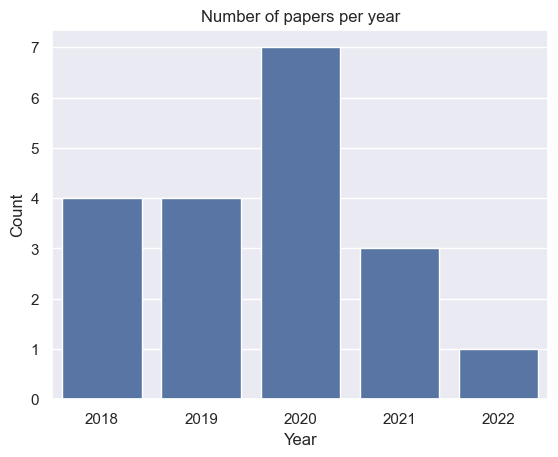
\includegraphics[width=0.5\textwidth]{figures/slr_result_year_paper.png}
\caption{Number of reviewed papers per year. \label{fig:slr_results_year}}
\end{figure}

\begin{figure}[ht]
\centering
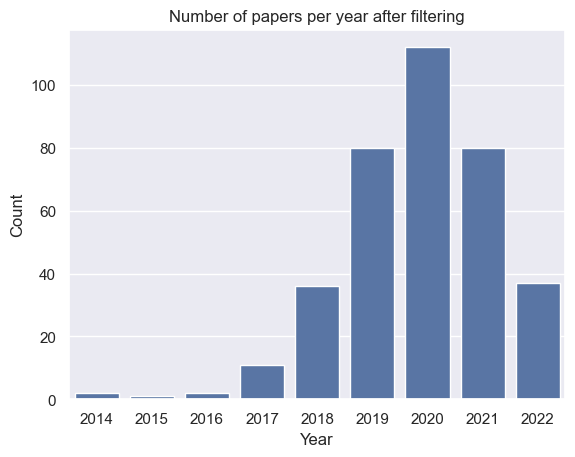
\includegraphics[width=0.5\textwidth]{figures/slr_results_filtering.png}
\caption{Number of reviewed papers after citation filter step (Fig. \ref{fig:slr_pipeline})}
\label{fig:slr_after_filter}
\end{figure}

Fig. \ref{fig:slr_results_year} shows the number of analysed papers per year, and Fig. \ref{fig:slr_after_filter} shows the year distribution of the papers analysed by hand after the application of the citation filter (Fig. \ref{fig:slr_pipeline}). The majority of the papers that were chosen were from 2020. Even after the restrictions applied to the search query, a significant portion of the results is still comprised of GANs for image synthesis.

Further analysis can be done with regard to the search questions defined in sec. \ref{sec:search_questions}. For \textbf{SQ1}, it was shown that several solutions apply GANs or variations in anomaly detection in tabular datasets. Surprisingly, some models worked on image and tabular datasets with the proper adjustments. Additionally, 40\% use either an autoencoder or parts of it to help with anomaly detection in complex data types and 9/20 use some variation of reconstruction errors to determine if a sample is anomalous.

As for \textbf{SQ2}, it was shown that most methods (75\%) learn the normal distribution during the training phase and then detect outliers. 20\% generate outliers that are used to train classifiers for detecting anomalies. Only \cite{wang.etal_AnomalyDetectionMinimum_2018} makes use of both abnormal and normal data distribution in the training phase. This indicates that most GAN-based solutions for anomaly detection can generate realistic data with the same distribution as the original data. However, not all use the discriminator to distinguish between normal and abnormal samples, as they employ classifiers.

\section{Threats to SLR}\label{sec:slr_threats}
The chosen limit for the minimum citations might have been too restrictive, especially for the papers recently published. The adaptation of inclusion criteria I4 (Table \ref{tab:criteria}) to allow for fewer citations in earlier papers was made to try and mitigate this risk. Despite this, the number of analysed papers for 2022 was significantly smaller than the previous years, which introduces the risk that some of the newer published relevant papers might have been overlooked. 

Furthermore, as only one search engine was used for the SLR, there is also the risk that some relevant papers from other platforms were not encountered during this process. 

Another threat may arise due to the terms used to search for relevant papers. After analysing multiple papers, various synonyms for both GANs and anomalies were collected to reach the most number of papers possible. Despite this, there exists the possibility that some authors didn't use any of these terms to characterize their approach in the title, abstract or keywords of the document. This way, there is a small risk that some relevant papers might have eluded the search query.

Similarly, by prohibiting documents that referenced images, or anything other than tabular data, some relevant papers might have been excluded. This can occur, for instance, in architectures that were firstly designed for image anomaly detection but were also suited for tabular datasets.

\section{Summary}\label{sec:summary}
This chapter explained the methodology used to aggregate the papers relevant to the problem in question. First, a set of search questions were defined (sec. \ref{sec:search_questions} followed by the respective query (sec. \ref{sec:search_queries} that was used on Scopus. The selection criteria and the processing pipeline were delined in Section \ref{sec:inclusion_exclusion}. A summary of each of the selected papers is provided in Section \ref{sec:stoa_results}. Next, a categorization and summary of the entire process are performed in Section \ref{sec:res_analysis}, followed by the threats to the SLR process (sec. \ref{sec:slr_threats}).


% TODO rever anomaly method para USAD
% TODO rever blance et al.




\chapter{Research Proposal}\label{chap:research_proposal}

This chapter will provide an overview of the problem this thesis is trying to solve. First, a brief analysis of the input data used by all methods will be presented in Section \ref*{sec:prelim_data_analysis}. Next, the existing methods for initial flow estimation will be presented in Sections \ref{sec:multivp} and \ref{sec:ml_initial_flow}. In Section \ref{sec:prelim_data_analysis}, a preliminary analysis of the input data used in both approaches is undertaken. With the problems identified in the previous section, a hypothesis and research questions are proposed in Section \ref{sec:hypothesis}, intending to solve these issues. Finally, the methodology and development plans are presented in Sections \ref{sec:method} and \ref{sec:work_plan}, respectively.

\section{Magnetogram Data}\label{sec:prelim_data_analysis}

The data used by all the methodologies consists of files with 640 entries ordered as the distance to the Sun. The data is divided into two parts: the input and the output. The input data comprises the magnetic field amplitude, $B$, the flux tube inclination, $\alpha$, and the radial coordinate, $R$. The output data includes the number of charged particles per unit volume, $n$, the velocity, $v$, and the temperature, $T$. Table \ref{tab:multivp_columns} presents the input and output data columns.

\begin{table}[ht]
    \caption{Data columns of magnetogram used by MULTI-VP.}
    \label{tab:multivp_columns}
    \begin{subtable}[h]{0.32\textwidth}
        \centering
        \begin{tabular}{lcc}
        \hline
        \multicolumn{3}{c}{Input (Partial Flows)}                              \\ \hline
        $R${[}$R_{sun}${]} & $B${[}$G${]} & $\alpha${[}$deg${]} \\ \hline
        \end{tabular}
    \end{subtable}
    \begin{subtable}[h]{0.32\textwidth}
        \centering
        \begin{tabular}{ccc}
        \hline
        \multicolumn{3}{c}{Output (Estimations)}                           \\ \hline
        $n${[}$cm^{-3}${]} & $v${[}$km/s${]} & $T${[}$MK${]} \\ \hline
        \end{tabular}
    \end{subtable}
\end{table}

Some preliminary analysis of the input data for the model was carried out to demonstrate the existence of anomalies in the data used to train the prediction model of the previous section. The radial profiles of the magnetic field in the function of the radial coordinate radius, $R$, can be seen in Fig. \ref{fig:magnetic_radius_outliers}. It is possible to observe some extreme variations in the data, which indicate the existence of abnormal samples. Additionally, the distribution of magnetic field, $B$, and flux tube inclination values, $\alpha$, are expressed in Figure \ref{fig:input_distrib_bp}. There exist a large number of out-of-distribution samples in the dataset used for training the prediction model.

A similar process was carried out on the output data (refer to Table \ref{tab:multivp_columns}) to assert if it contained abnormal values that would also affect the training of the ML solution. Significant fluctuations can be observed in all instances of the output columns in Figure \ref{fig:output_distr_plot}. The distribution for the output values can also be seen in Figure \ref{fig:output_distrib_bp}.

\begin{figure}[ht]
\centering
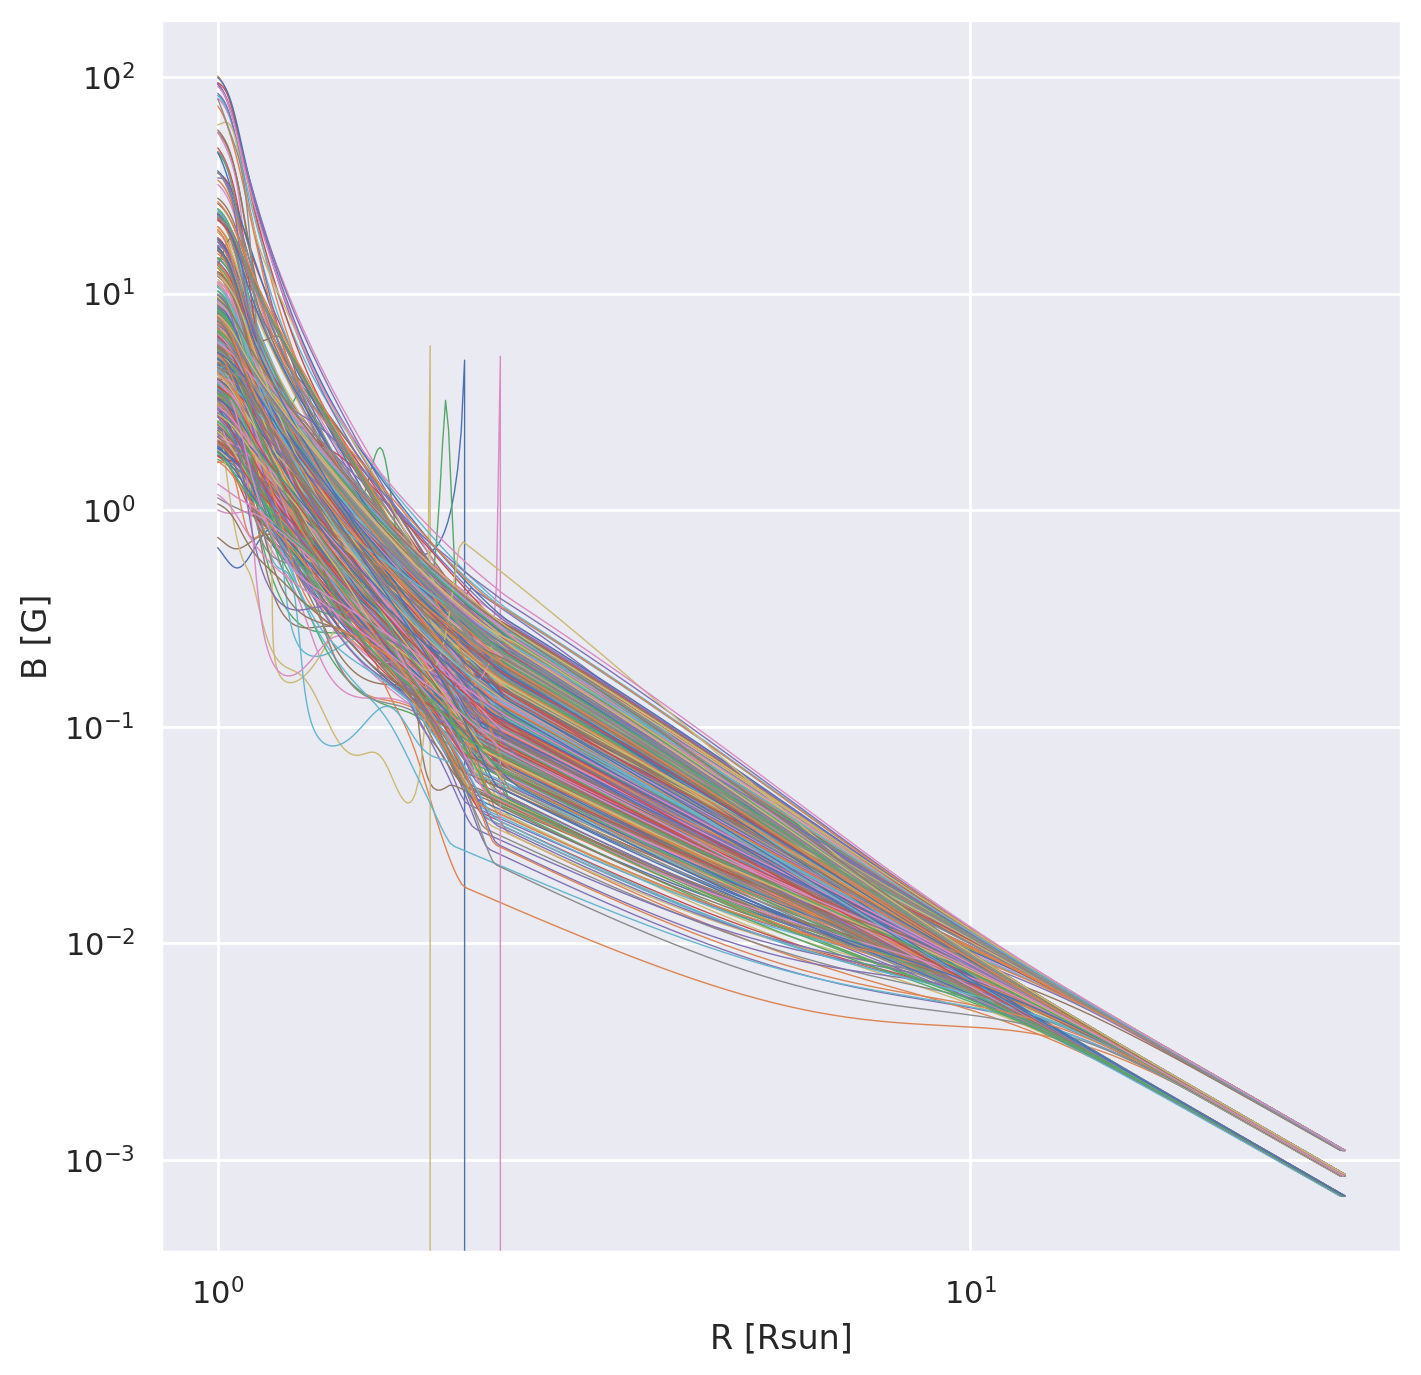
\includegraphics[width=0.5\textwidth]{figures/magnetic_radius_outliers.png}
\caption{Radial profiles of the magnetic field amplitude for the dataset flux-tubes.}
\label{fig:magnetic_radius_outliers}
\end{figure}

\begin{figure}[ht]
     \centering
     \begin{subfigure}[b]{0.32\textwidth}
         \centering
         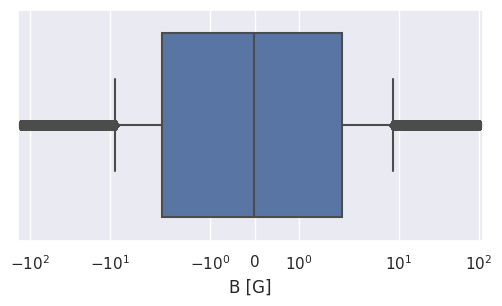
\includegraphics[width=\textwidth]{figures/magnetic_field_boxplot.png}
     \end{subfigure}
     \hfill
     \begin{subfigure}[b]{0.32\textwidth}
         \centering
         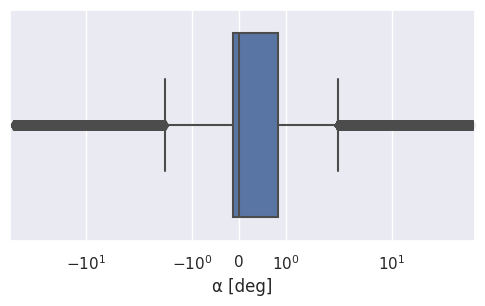
\includegraphics[width=\textwidth]{figures/inclination_bp.png}
     \end{subfigure}
     \hfill
        \caption{Distribution of input values}
        \label{fig:input_distrib_bp}
\end{figure}


\begin{figure}[!ht]
     \centering
     \begin{subfigure}[b]{0.32\textwidth}
         \centering
         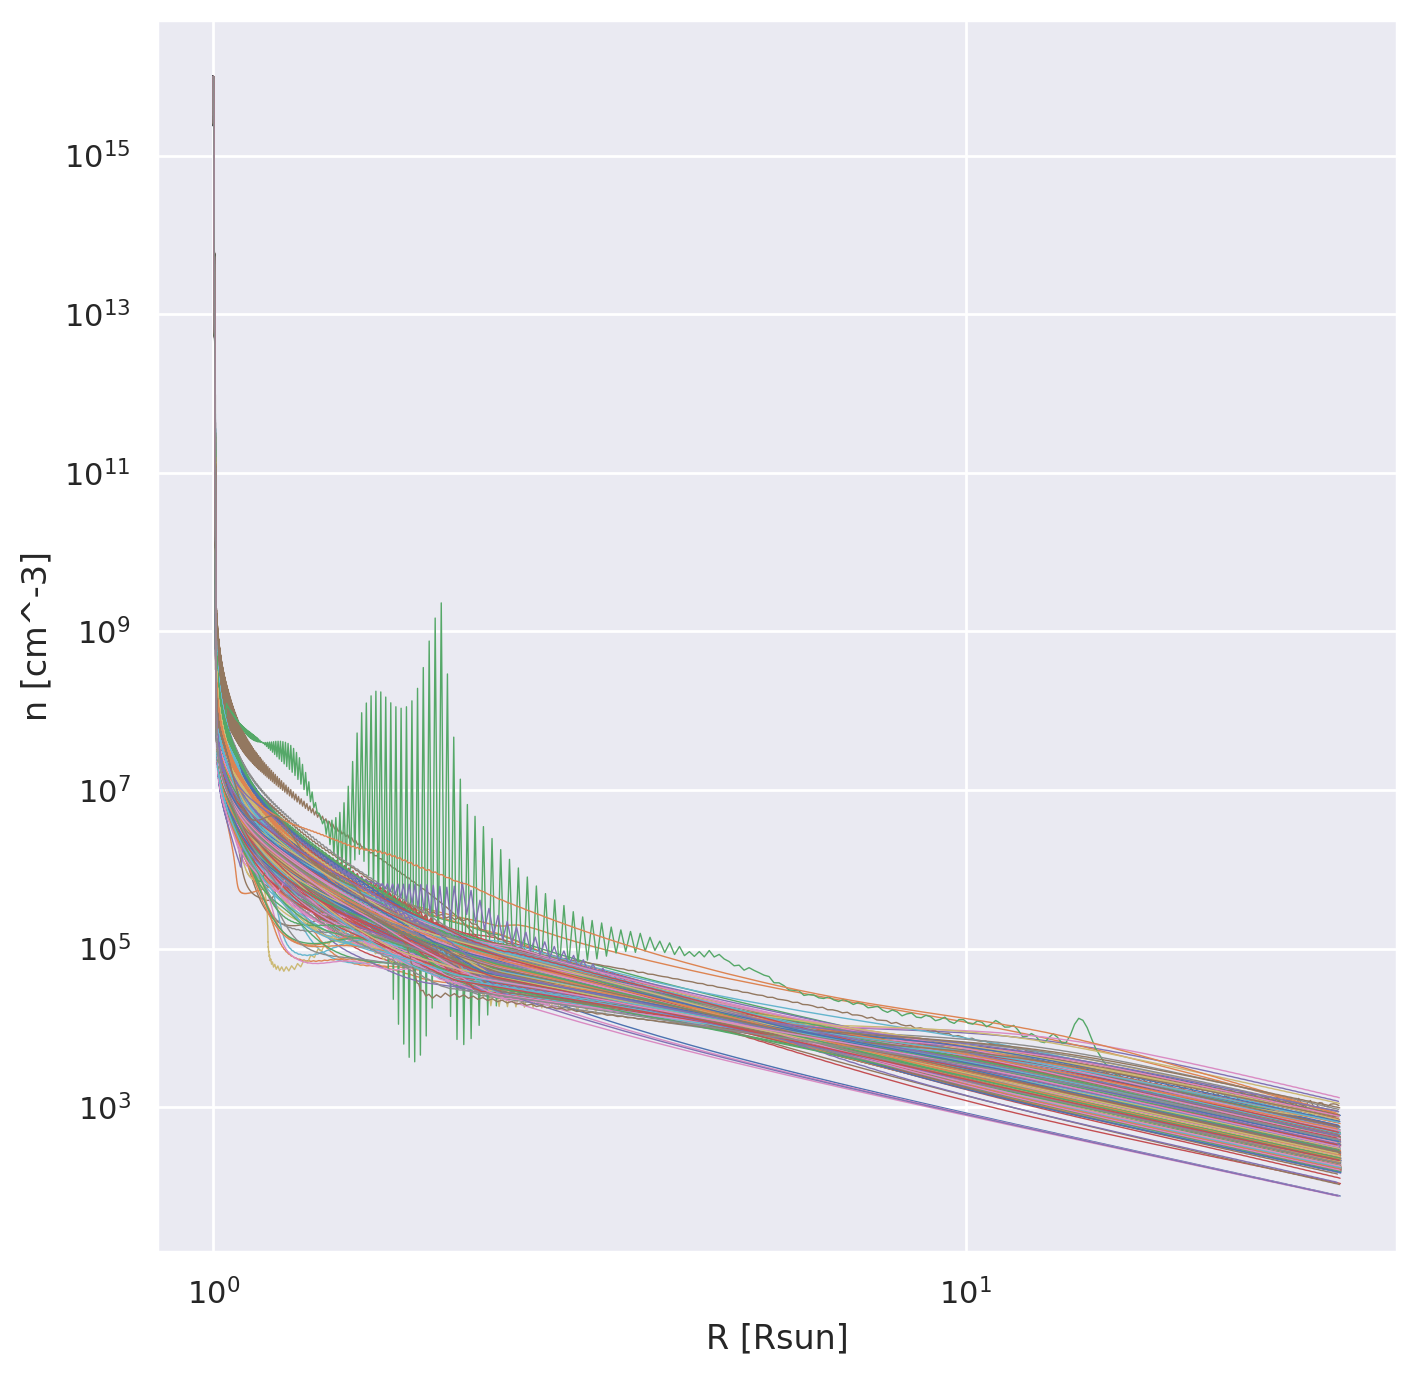
\includegraphics[width=\textwidth]{figures/volume_radius.png}
     \end{subfigure}
     \hfill
     \begin{subfigure}[b]{0.32\textwidth}
         \centering
         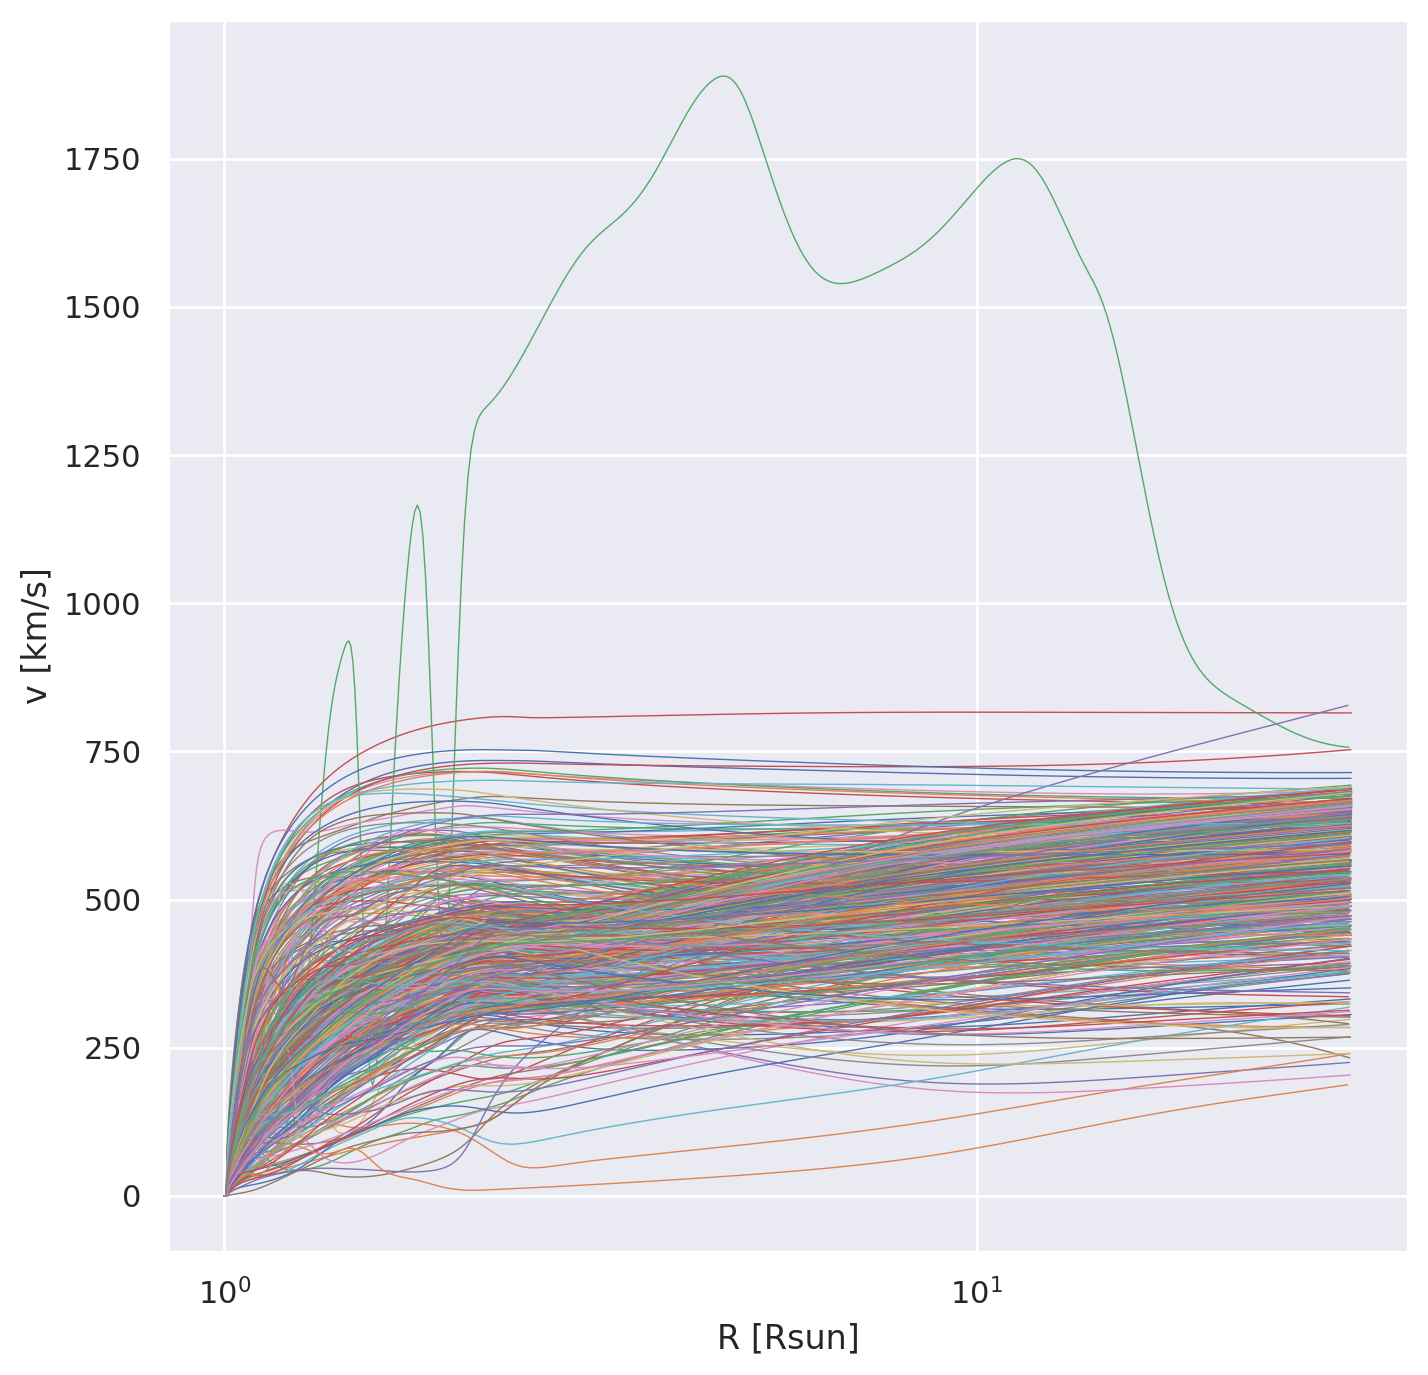
\includegraphics[width=\textwidth]{figures/velocity_radius.png}
     \end{subfigure}
     \hfill
    \begin{subfigure}[b]{0.32\textwidth}
         \centering
         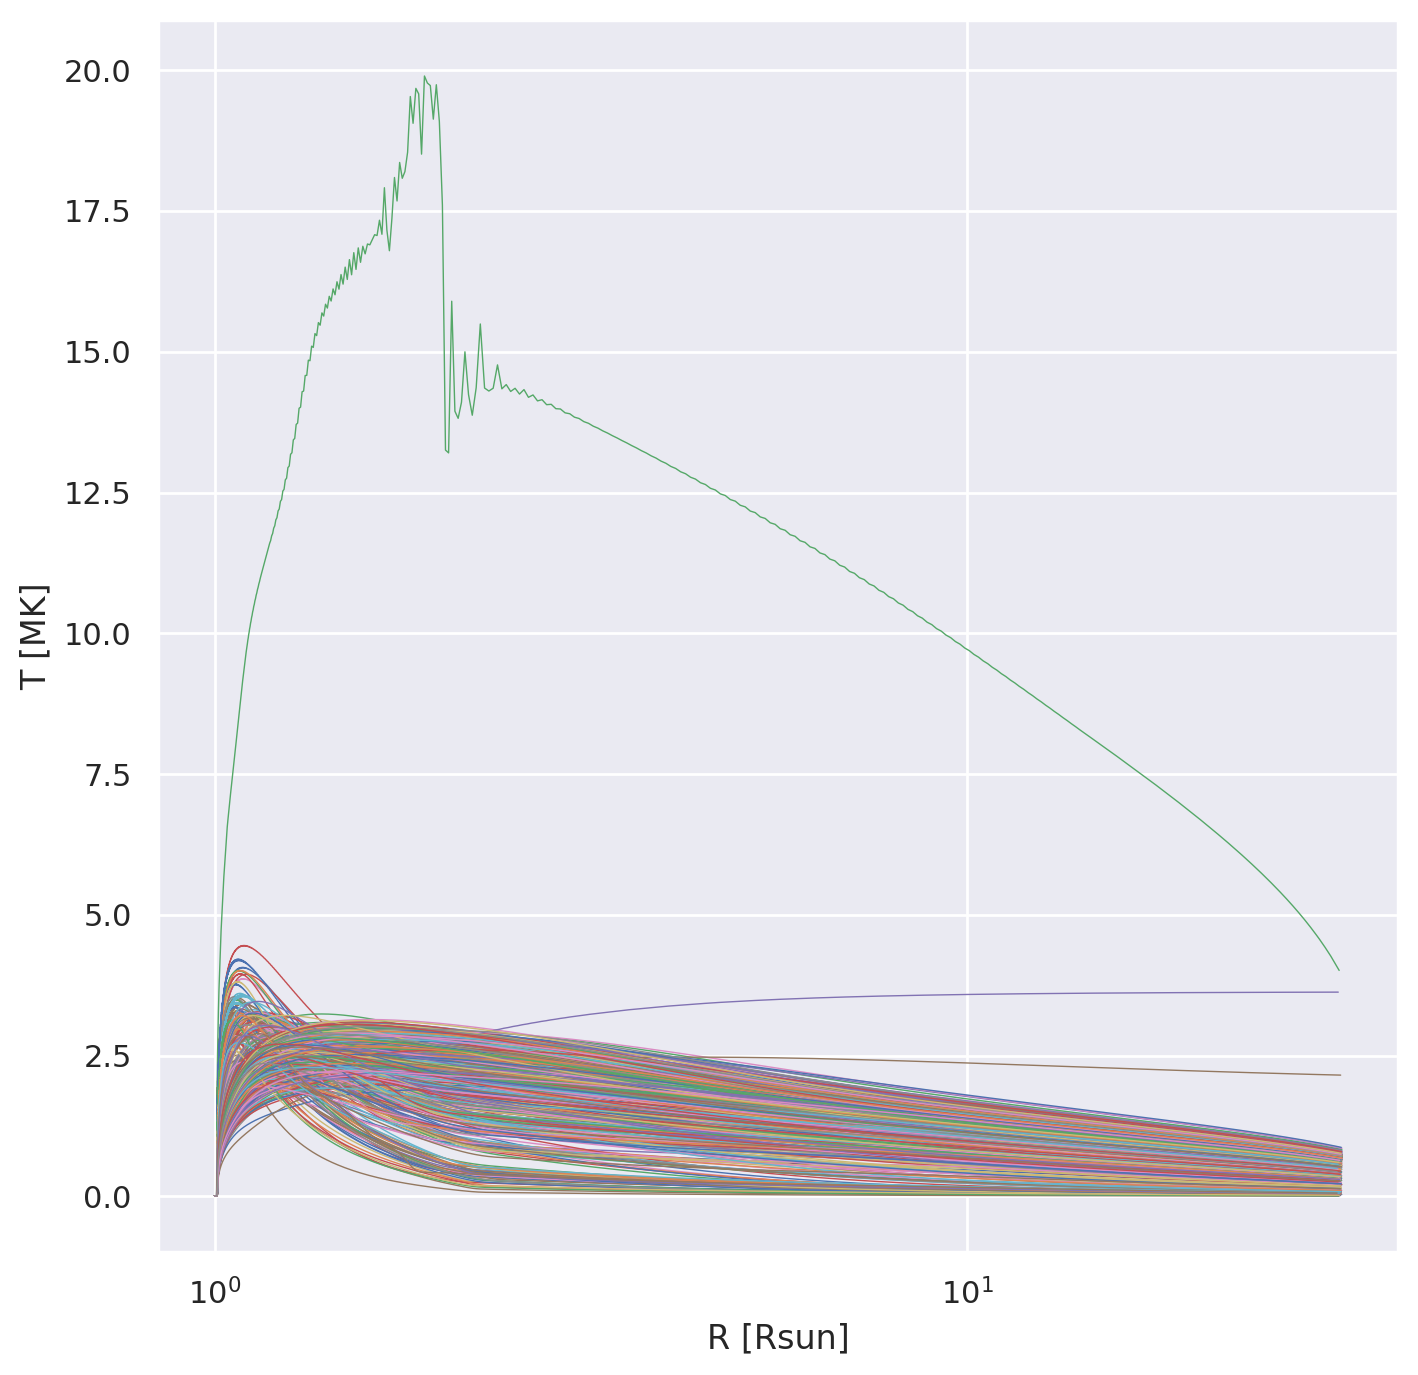
\includegraphics[width=\textwidth]{figures/temperature_radius.png}
     \end{subfigure}
     \hfill
    \caption{Plots of output variables in relation to $R$.}
    \label{fig:output_distr_plot}
\end{figure}

\begin{figure}[!ht]
     \centering
     \begin{subfigure}[b]{0.32\textwidth}
         \centering
         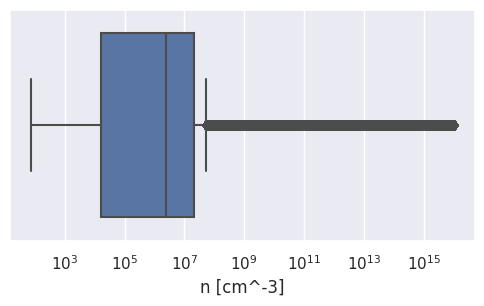
\includegraphics[width=\textwidth]{figures/volume_bp.png}
     \end{subfigure}
     \hfill
     \begin{subfigure}[b]{0.32\textwidth}
         \centering
         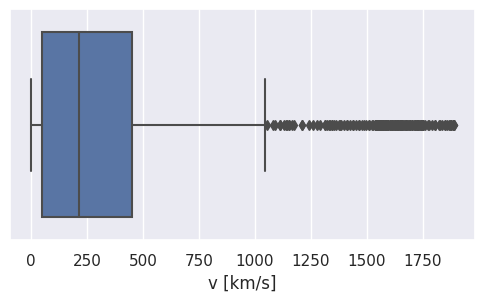
\includegraphics[width=\textwidth]{figures/velocity_bp.png}
     \end{subfigure}
     \hfill
     \begin{subfigure}[b]{0.32\textwidth}
         \centering
         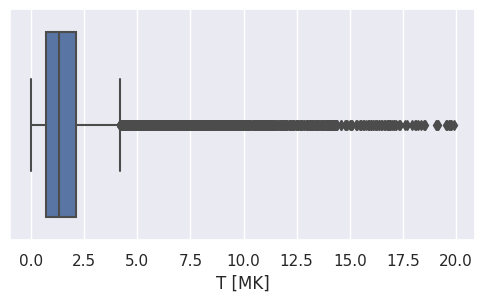
\includegraphics[width=\textwidth]{figures/temperature_bp.png}
     \end{subfigure}
     \hfill
        \caption{Distribution of outputs used during the training of the predictive model.}
        \label{fig:output_distrib_bp}
\end{figure}


\section{MULTI-VP}\label{sec:multivp}

MULTI-VP \cite{pinto.rouillard_MultipleFluxtubeSolar_2017} is a global MHD model that simulates the three-dimensional structures of the solar wind. In addition, it also estimates the conditions at the Sun's chromosphere, transition region, corona, and low heliosphere. The model computes many one-dimension solar wind solutions from full flux-tube geometries and heating functions. Background magnetic field geometries are extrapolated from publicly available magnetogram data. The method can estimate solar wind profiles across the Sun's entire atmosphere up to 30 solar radii. The results directly link the geometry of magnetic flux tubes in the lower corona with the distributions of fast and slow solar wind flows. MULI-VP proved faster than other MHD models and did not suffer from cross-field diffusion effects.

The data used as input to the model is presented in Table \ref{tab:multivp_columns}. A representation of the data processing of MULTI-VP can be seen in Figure \ref{fig:multivp_method}. As previously stated, MULTI-VP takes as input partial flow definitions of the solar wind along with initial expert estimations and derives better solutions during simulation.

\vspace{0.5cm}
\begin{figure}[!h]
\centering
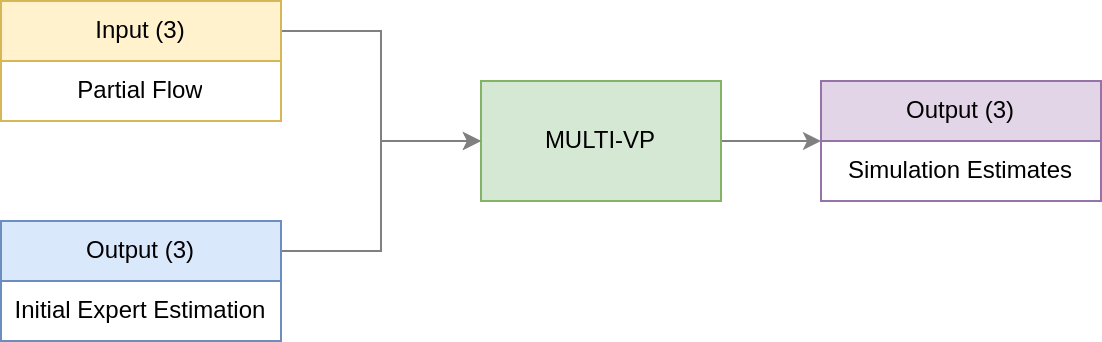
\includegraphics[width=0.8\textwidth]{figures/multivp_method.png}
\caption[MULTI-VP methodology dataflow]{MULTI-VP methodology dataflow. The model takes as input both the partial flow and its associated expert initial guess and then derives a better solution.\label{fig:multivp_method}}
\end{figure}


\section{ML for Initial Flow Estimation}\label{sec:ml_initial_flow}
Due to the complexity and a large number of calculations, MULTI-VP, like other MHD simulations, still takes a long time to reach solar wind solutions. Furthermore, the need for initial expert guesses also significantly delays the process. These factors directly affect the prediction capability and preparation for extreme solar events. Recently in \cite{barros_InitialConditionEstimation_}, it has been proved that machine learning techniques can accurately produce good initial flow estimations that MULTI-VP can later use. The authors also proved that the quality of the flow estimations is directly linked to the total execution time of the simulation. These allow for faster convergence of the MHD simulation as the initial estimates are closer to the final solution. 

The approach, illustrated in Fig. \ref{fig:multivp_rnn}, uses an ML model to predict the initial expert estimates from the initial partial flow input. Analogous to the method presented in Section \ref{sec:multivp}, MULTI-VP takes as input the partial flows along with their initial conditions predicted by the ML model.

An illustration of the training method can be seen in Figure \ref*{fig:rnn_train}. In this phase, the model takes as inputs initial partial flows and tries to predict the initial estimations. Next, the predictions for a given flow are compared to those from previous MULTI-VP runs to calculate the prediction's loss and update the model's parameters with backpropagation. The logic behind this was that the model would learn to predict initial estimations closer to the final solution, and thus, the simulation would converge faster.

\begin{figure}[ht]
\centering
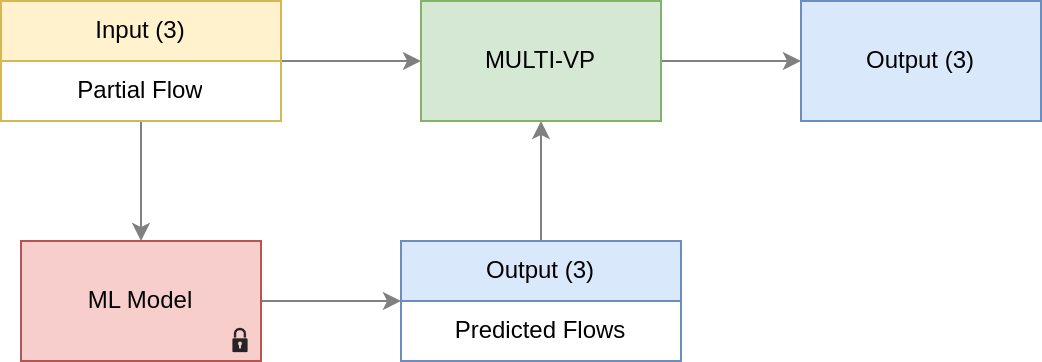
\includegraphics[width=0.8\textwidth]{figures/multivp_rnn.png}
\caption[ML methodology dataflow]{ML methodology dataflow. An ML model estimates the initial conditions of a given partial flow. These are then passed to MULTI-VP, approximating them into a final solution. \label{fig:multivp_rnn}}
\end{figure}

\begin{figure}[!ht]
    \centering
    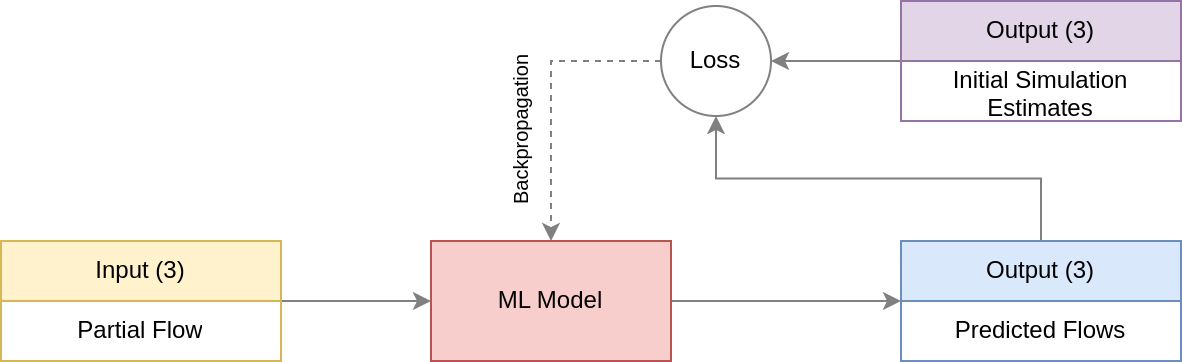
\includegraphics[width=0.8\textwidth]{figures/rnn_training.png}
    \caption[ML training phase]{Model training method. Takes as input initial partial flows and tries to predict flow estimates close to the ones from previous MULTI-VP simulations.\label{fig:rnn_train}}
\end{figure}

However, the reduction in execution time was minimal as the model, like many other ANN solutions, was very susceptible to noise in the samples used during training. In \cite{barros_InitialConditionEstimation_}, the authors posit that the presence of outliers during the training phase hampered the overall prediction quality of the model.


\section{Hypothesis}\label{sec:hypothesis}
Having these problems into consideration, this thesis aims to evaluate the following hypothesis:
\begin{adjustwidth}{2cm}{}
    GAN-based anomaly detection architectures can accurately and automatically detect outliers in the solar wind profiles data used to train the NN model for initial condition estimation and improve the model's predictions.
\end{adjustwidth}

We will try to validate this hypothesis by (1) verifying that the dataset after outlier removal significantly improves the prediction quality of the RNN and (2) if the predictions with a normalized dataset reduce the time that MULTI-VP takes to reach a solution.

To validate the above hypothesis, the following research questions were defined:

\begin{description}
    \item[RQ1] \textit{Can GAN-based architectures accurately detect outliers in solar wind profiles?} Considering outlier samples as the positive class, we are mostly trying to reduce the False Negative Rate (FN), which causes the worst effects in the predictive model training. As a secondary priority, we will focus on reducing the amount of False Positives (FP) to ensure that almost no relevant samples are excluded from the training process.
    \item[RQ2] \textit{Does the resulting dataset significantly improve the predictive ability of the RNN?} If the resulting dataset after the removal of outliers results in an improvement in the model used to predict initial conditions from input flows. In other words, the mean square distance between the real estimations and the ones predicted by the model is less than with the previous method.
    \item[RQ3] \textit{Does the improved predictive ability of the RNN result in a further reduction of execution time for MULTI-VP?} This question aims to clarify if the developed model for initial flow estimation can produce better approximations of solar wind flows and thus reduce the time it takes for MULTI-VP to reach a solution.
\end{description}

\section{Methodology}\label{sec:method}
To evaluate the integrity of the hypothesis, we propose developing a GAN architecture to detect outliers in magnetogram files with an approach similar to the ones in \cite{li.etal_MADGANMultivariateAnomaly_2019}, and \cite{bashar.nayak_TAnoGANTimeSeries_2020}. It will use the generator and the discriminator to detect anomalies in the dataset. 

The developed anomaly detector will be incorporated into the existing ML methodology expressed in Figure \ref{fig:multivp_rnn}. The resulting representation of the overall data flow for the proposed approach can be seen in Figure \ref{fig:gan_rnn_multivp}. The goal is to use a GAN-based solution to detect outlier samples before training the ML models for initial flow estimation. We propose using the input values of the available magnetograms for this step. The detected anomalies will be removed from the dataset, and the RNN model will be trained with the remaining samples. The new predictions will be compared to the ones from the previous method to evaluate the improvement in the prediction quality. Finally, the predictions will be used as initial conditions for MULTI-VP, and the execution time will be compared to the previous method.

\begin{figure}[ht]
\centering
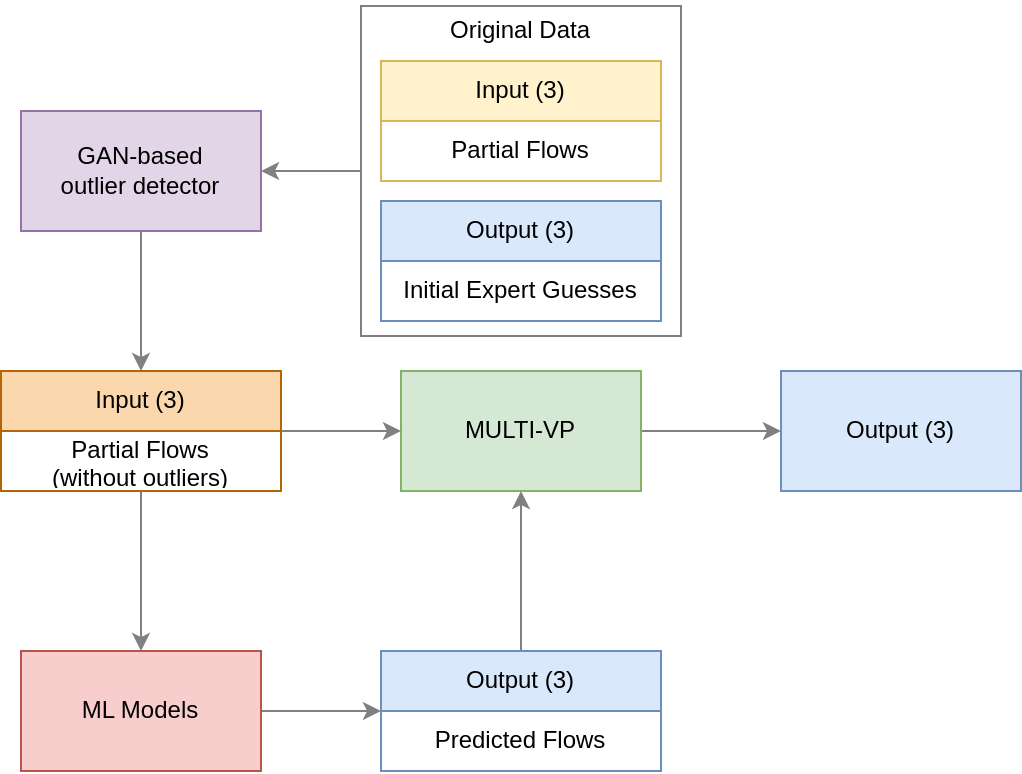
\includegraphics[width=0.8\textwidth]{figures/gan_rnn_multivp.png}
\caption{GAN-based outlier detection method dataflow.}
\label{fig:gan_rnn_multivp}
\end{figure}

The GAN will have a similar architecture to the one in \cite{goodfellow.etal_GenerativeAdversarialNets_}. During training (Fig. \ref{fig:proposed_gan_train}), the generator's goal is to synthesize magnetogram samples close to the original distribution of the dataset. The discriminator will be tasked with distinguishing fake magnetograms from real ones. %Only normal samples will be used in this process.

\begin{figure}[ht]
    \centering
    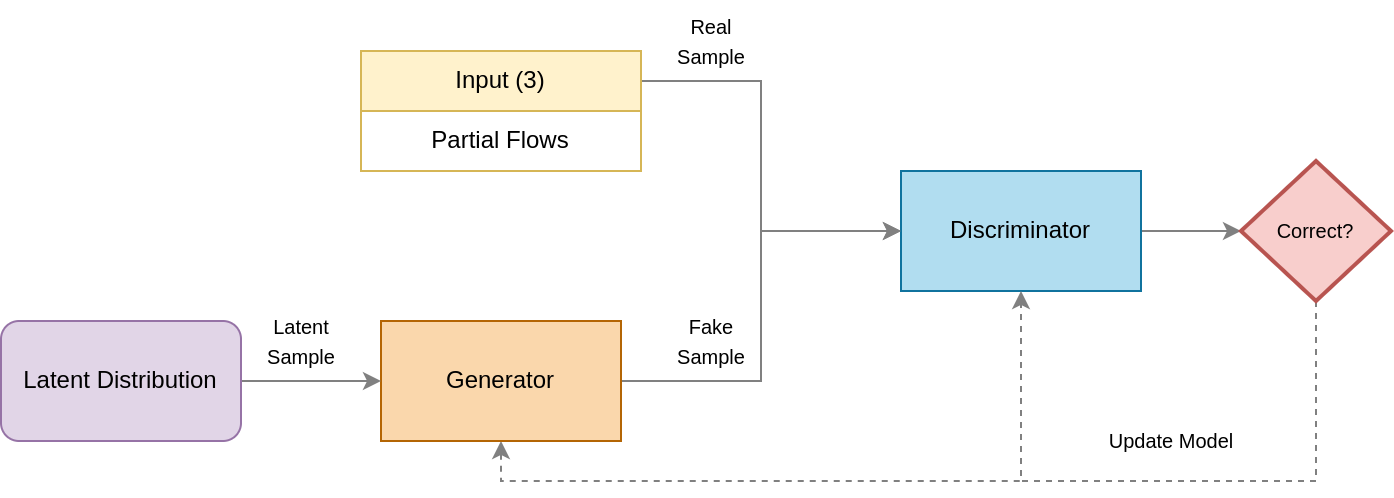
\includegraphics[width=0.8\textwidth]{figures/gan_arch_train.png}
    \caption{Proposed training method.}
    \label{fig:proposed_gan_train}
\end{figure}

For the detection phase, we propose the methodology in Figure \ref{fig:proposed_gan_arch} with the components trained in the previous stage. First, a sample will be extracted from the dataset and passed directly to the discriminator. If the sample is abnormal, it will most likely have a higher loss than normal ones, as the discriminator only retained the normal data distribution. Next, the sample is mapped into the latent space, where one of the methods from \cite{li.etal_MADGANMultivariateAnomaly_2019} or \cite{bashar.nayak_TAnoGANTimeSeries_2020} could be used. The resulting latent sample is then fed to the generator, which is tasked with reconstructing it. In the next step, the reconstructed sample is compared with the real one, and the reconstruction error is calculated. In theory, if the real sample is defective, then the reconstruction error will be much higher when compared to normal examples, as the generator only learned to generate samples from the normal distribution. In the end, discriminator loss and the reconstruction error will be combined to calculate the anomaly score. The example is considered an anomaly if this score exceeds a predefined threshold.

\begin{figure}[ht]
\centering
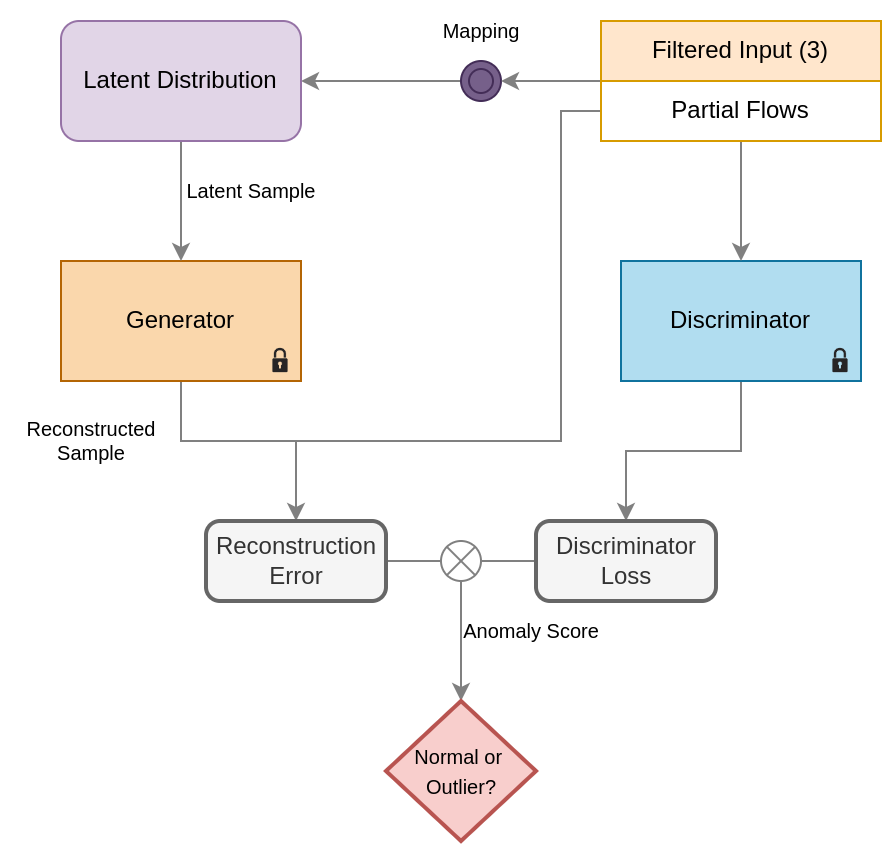
\includegraphics[width=0.8\textwidth]{figures/proposed_gan_arch.png}
\caption{Proposed method for anomaly detection in magnetogram data.}
\label{fig:proposed_gan_arch}
\end{figure}


The results will be evaluated in an initial step by comparing the distance between the predicted initial estimation of the ML model and the real ones. Similar to the work carried out in \cite{barros_InitialConditionEstimation_}, we will measure the Mean Squared Error (MSE) between the two. Subsequently, the filtered inputs from the outlier detection step will be fed to MULTI-VP along with the initial flow estimations from the ML model. Then the simulation execution times when using the proposed methodology will be compared with the previous implementations to assert if there was a significant reduction.

\section{Work Plan}\label{sec:work_plan}
In Figure \ref{fig:work_plan}, an illustration of the proposed work plan is given. In the initial part of development, a more in-depth analysis of the input data will be performed. In addition, we will try to apply some clustering methods to determine if any subgroups in the dataset would facilitate the anomaly detection method.

In the next stage, a GAN architecture will be designed to detect outliers in magnetogram data. Pytorch \cite{NEURIPS2019_9015} will be the tool used for this goal. Some time was also allocated to implementing GANs with this framework. After developing a suitable method for outlier detection on the given dataset, an extensive analysis of the performance of the ML model with the data without outliers will be done. This part will be used to validate the hypothesis defined in Section \ref{sec:hypothesis}. During this time, some adjustments might have to be made to the initial solution to overcome any shortcomings on these tests. As was already stated, we will use the MSE between the actual estimations and those predicted with the new method. 

After finetuning, the newly improved estimations from the previous step will be used on MULTI-VP to evaluate if the chosen implementation resulted in a shorter execution time. The final stage will be dedicated to writing the dissertation and accommodating any delays from the previous steps.

\begin{figure}[ht]
\centering
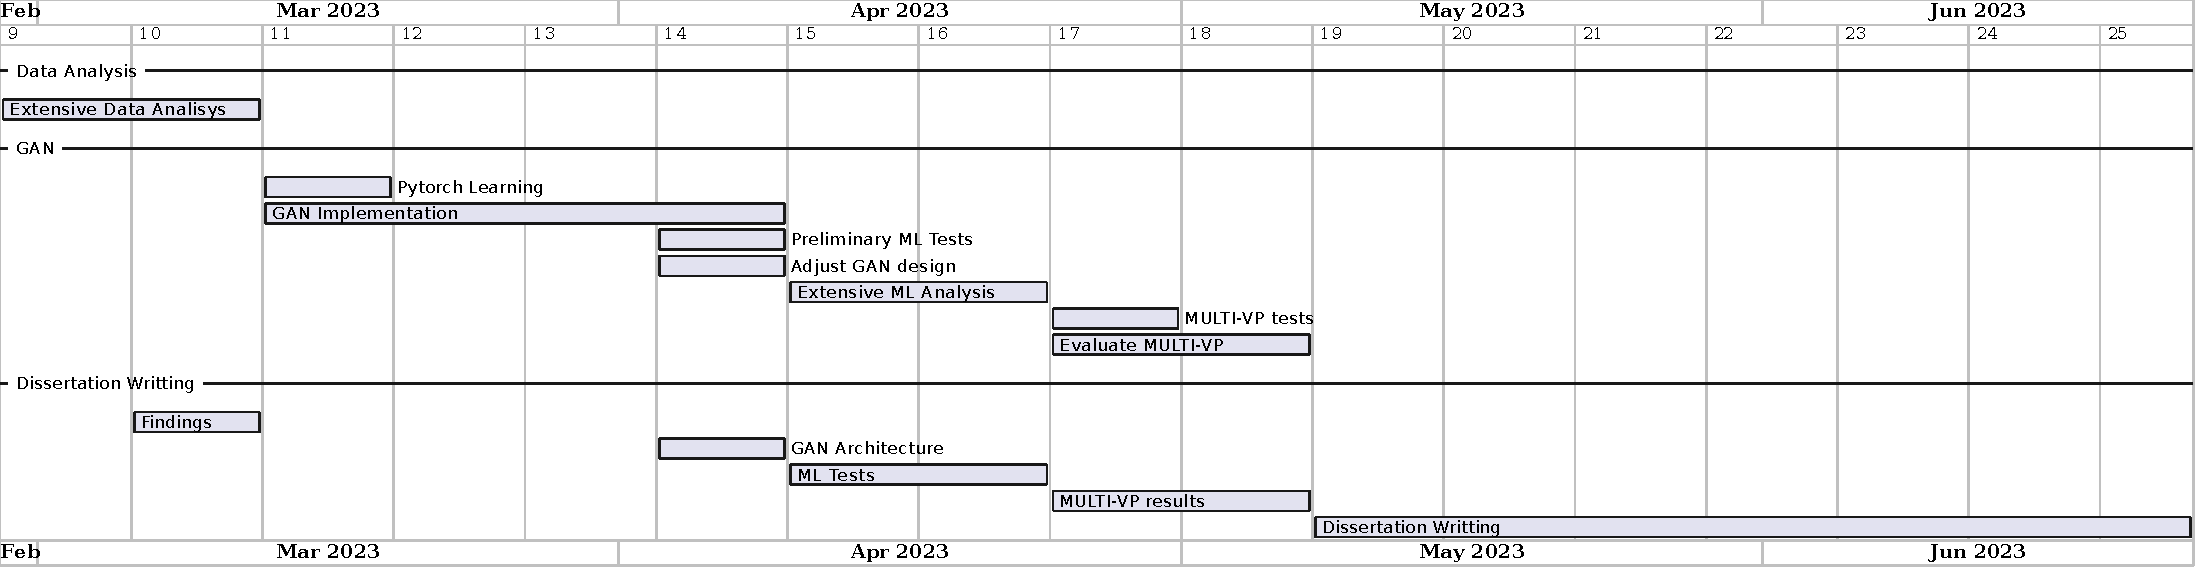
\includegraphics[width=\textwidth]{figures/work_plan.pdf}
\caption{Proposed development plan.}
\label{fig:work_plan}
\end{figure}

\chapter*{Exploratory Data Analysis}\label{chap:eda}
An extensive analysis of the data that will be used during the development process was carried out. This chapter presents the results of this analysis, which are used to guide the development of the system.


\section{Preliminary Analysis}\label{sec:data_prelim_analysis}
The data used by MULTI-VP and, consequently, the RNN prediction model consists of magnetogram data from the Wilcox Solar Observatory. Each file contains 12 columns representing measurements of the magnetic field in the solar atmosphere at different heights. Every variable comprises 640 points (abscissas) measured at different radial distances from the Sun (up to 30 Solar radii). For this work, only six columns will be used, as the others are derivations of these and, thus, are significantly correlated. 

The data columns can be seen in Table \ref{tab:multivp_columns}. These are divided into two parts: the input and the output. The former comprises the set of variables used by the simulation to approximate solar wind conditions, while the former consists of the initial expert guesses needed to kickstart the multiple flux simulation. The input data comprises the magnetic field amplitude, $B$, the flux tube inclination, $\alpha$, and the radial coordinate, $R$. The output data includes the number of charged particles per unit volume, $n$, the velocity, $v$, and the temperature, $T$.

\begin{table}[ht]
    \caption{Data columns of magnetogram used by MULTI-VP.}
    \label{tab:multivp_columns}
    \begin{subtable}[h]{0.32\textwidth}
        \centering
        \begin{tabular}{lcc}
        \hline
        \multicolumn{3}{c}{Input (Partial Flows)}                              \\ \hline
        $R${[}$R_{sun}${]} & $B${[}$G${]} & $\alpha${[}$deg${]} \\ \hline
        \end{tabular}
    \end{subtable}
    \begin{subtable}[h]{0.32\textwidth}
        \centering
        \begin{tabular}{ccc}
        \hline
        \multicolumn{3}{c}{Output (Estimations)}                           \\ \hline
        $n${[}$cm^{-3}${]} & $v${[}$km/s${]} & $T${[}$MK${]} \\ \hline
        \end{tabular}
    \end{subtable}
\end{table}

A joint plot of the input variables can be seen in Fig. \ref{fig:jointplot_input}. From these plots, it can be concluded that several input files constitute anomalous data. This is clear from the graphs of $B$ and $\alpha$, with files that significantly deviate from the rest.


\begin{figure}[h]
    \centering
    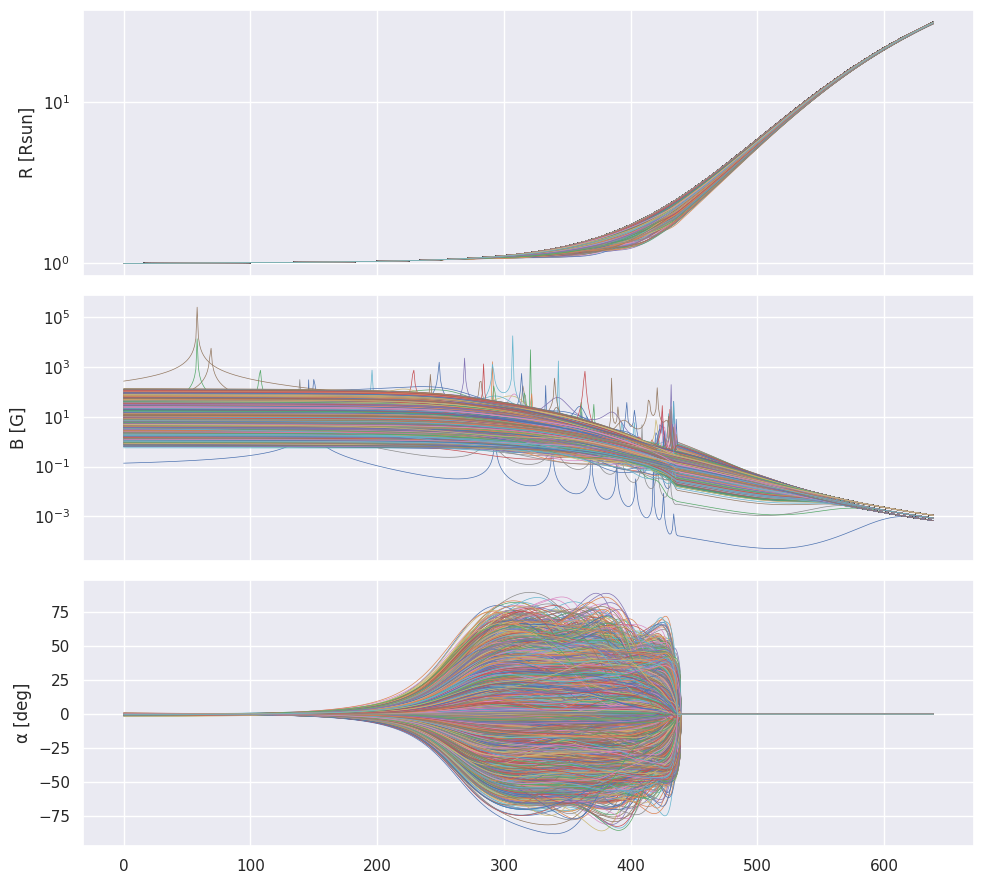
\includegraphics[width=0.8\textwidth]{figures/joint_input_cols.png}
    \caption{Joint plot of the input variables of each file used in this work. The first row is the plot of the radial coordinate radius, $R$, the second the magnetic field, $B$, and the last the flux tube inclination $\alpha$. All are plotted in function of position in the magnetogram file.}
    \label{fig:jointplot_input}
\end{figure}

% TODO refs para research statement
As previously explained, MULTI-VP requires initial expert guesses to kickstart the simulation. These guesses consist of the output variables presented in Table \ref{tab:multivp_columns} and, during the simulation, are approximated to better solutions. In line with the work carried out in \cite{barros_InitialConditionEstimation_}, we will be using the outputs of previous simulations as initial guesses (refer to chapter \ref{chap:research_proposal} for more details).


Fig. \ref{fig:jointplot_output} shows the joint plot of the output variables. Similar to the input plots, several faulty predictions can be seen in all variable plots, which are the result of simulations carried out on anomalous inputs.

\begin{figure}[h]
    \centering
    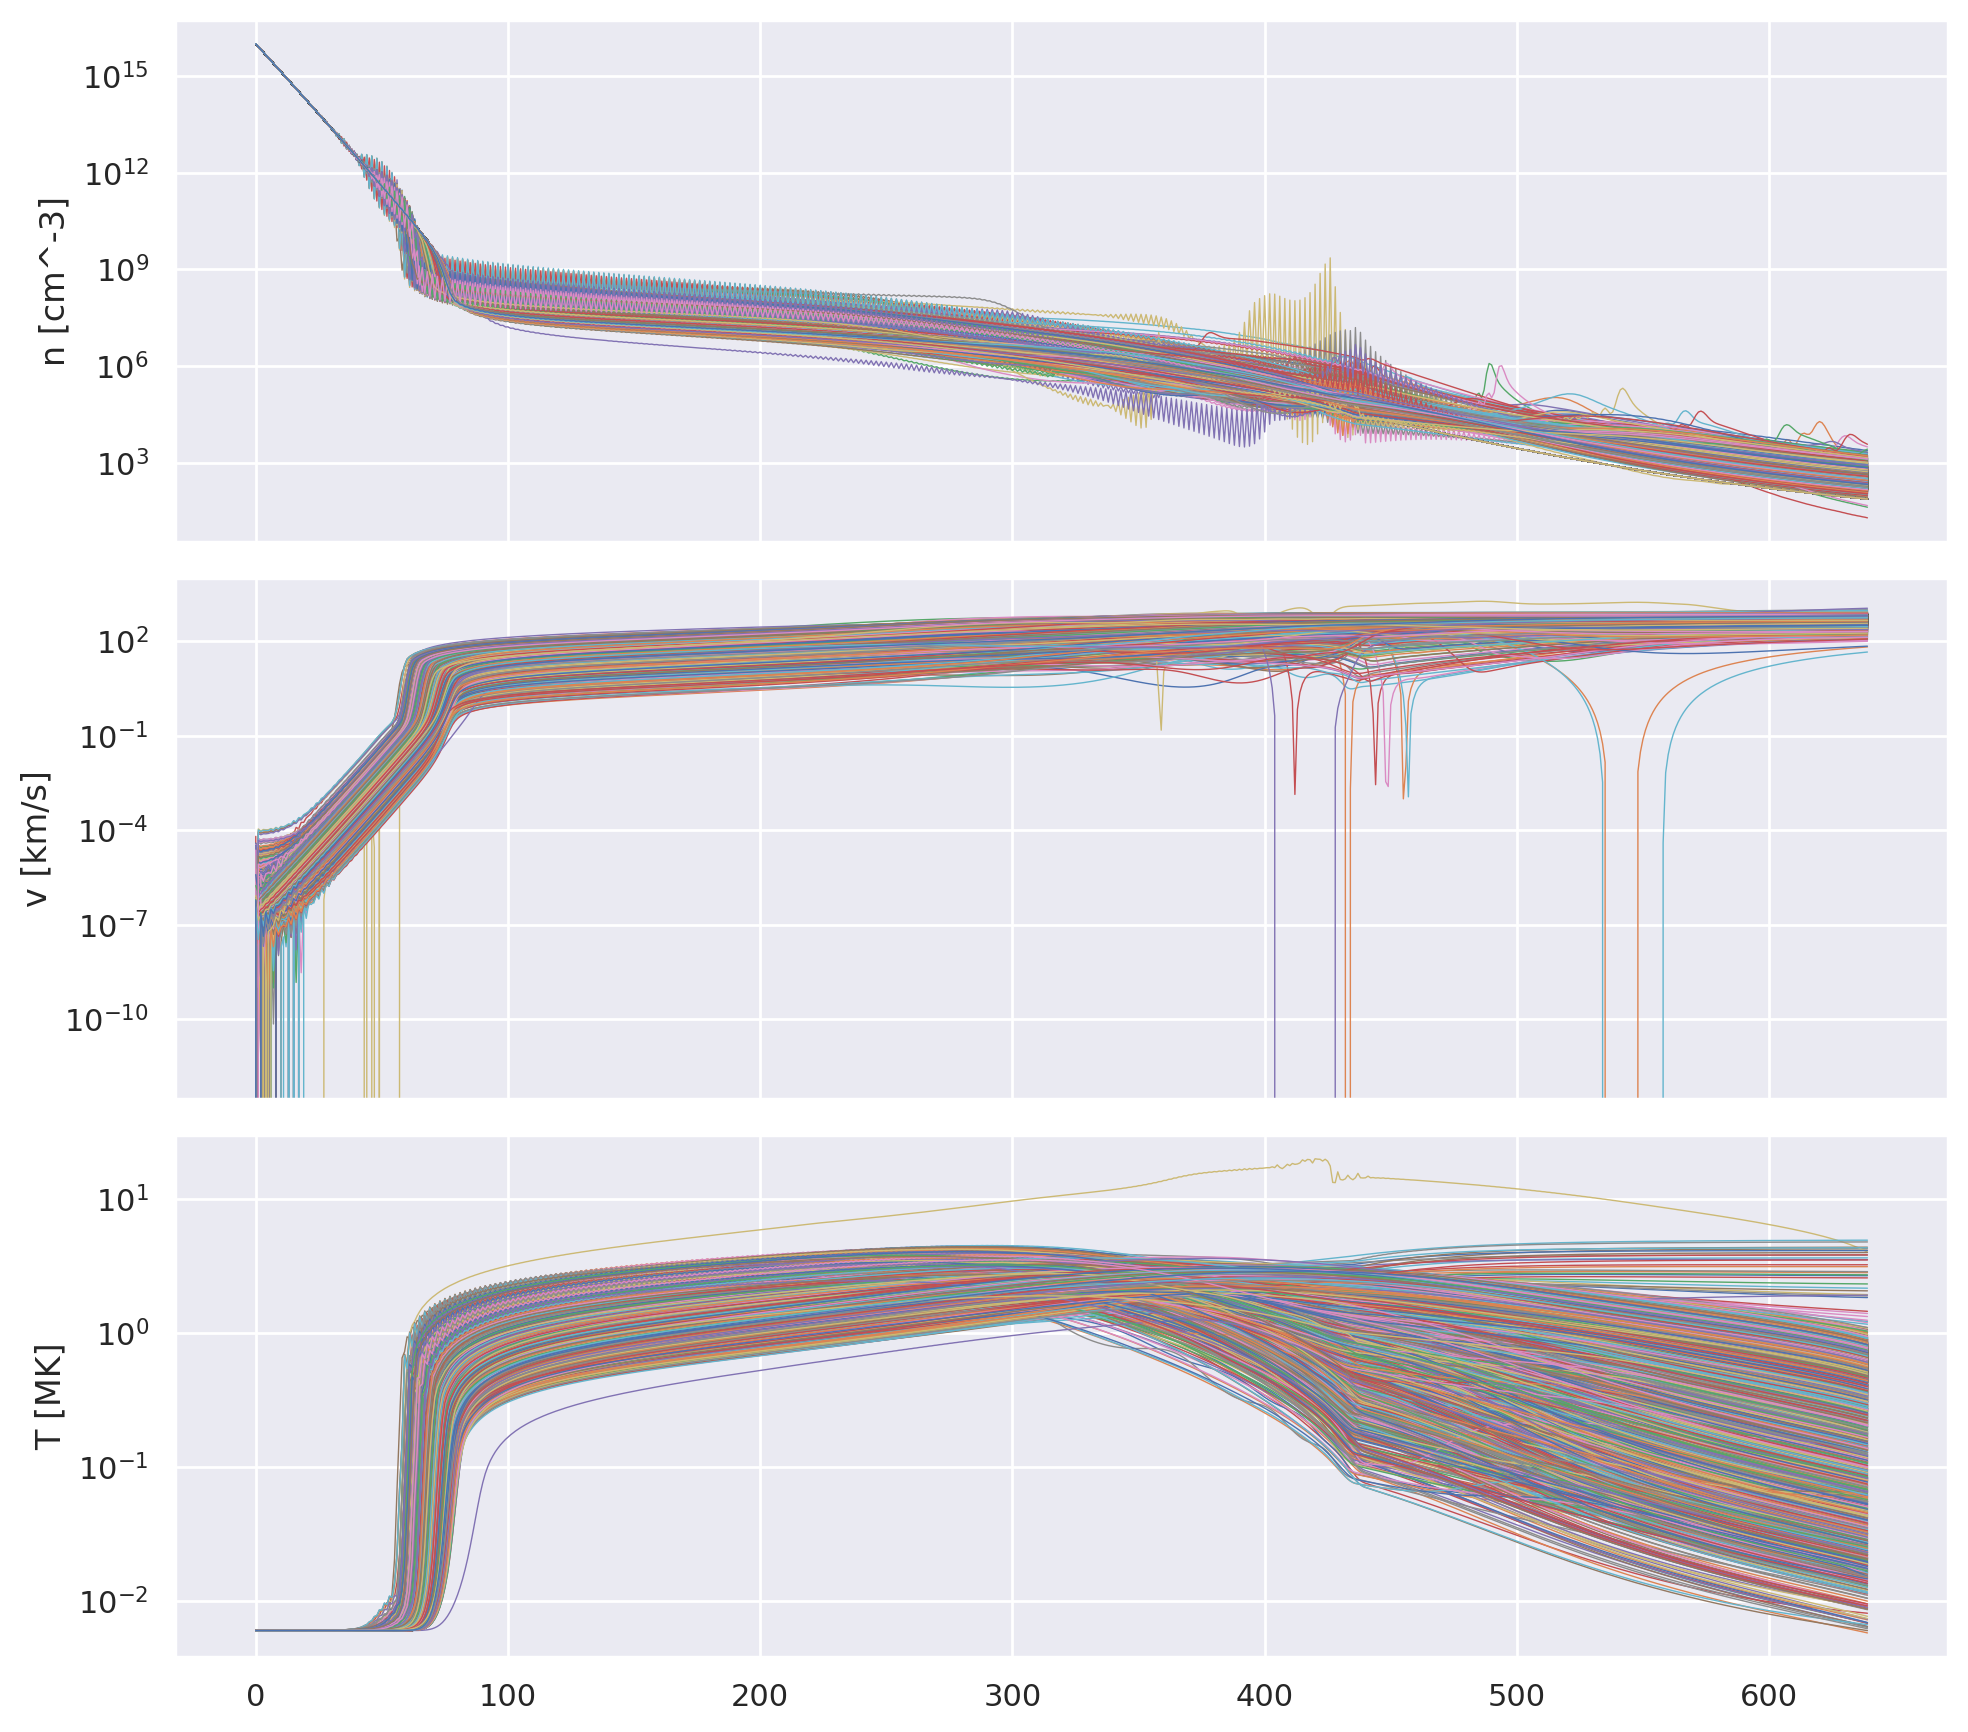
\includegraphics[width=0.8\textwidth]{figures/joint_output_cols.png}
    \caption{Joint plot of the output variables of each file used in this work. The first row is the plot of the number of charged particles per unit volume, $n$, the second the velocity, $v$, and the last the temperature, $T$. All are plotted in function of position in the magnetogram file.}
    \label{fig:jointplot_output}
\end{figure}

A preliminary statistical analysis of the data can be seen in tables \ref{tab:data_stats}. In it, the mean, standard deviation, minimum, maximum, and quartiles of each variable are presented.

\begin{table}[h]
    \caption{Data Statistical Analysis}
    \label{tab:data_stats}
    \begin{tabular}{@{}rrrrrrr@{}}
    \toprule
    \textbf{} & \textbf{R {[}Rsun{]}} & \textbf{B {[}G{]}} & \textbf{alpha {[}deg{]}} & \textbf{n {[}cm\textasciicircum{}-3{]}} & \textbf{v {[}km/s{]}} & \textbf{T {[}MK{]}} \\ \midrule
    mean      & 4.755                 & -0.536             & 1.885                    & 8.630207e+13                            & 255.325               & 1.384               \\
    std       & 7.165                 & 91.948             & 14.728                   & 6.839549e+14                            & 214.855               & 0.897               \\
    min       & 1.000                 & -17541.107         & -87.632                  & 1.972793e+01                            & -0.007                & 0.006               \\
    $25\%$    & 1.021                 & -2.145             & -0.108                   & 1.622396e+04                            & 49.263                & 0.718               \\
    $50\%$    & 1.151                 & 0.001              & 0.000                    & 2.350818e+06                            & 211.022               & 1.337               \\
    $75\%$    & 4.250                 & 2.054              & 1.000                    & 2.131588e+07                            & 450.770               & 2.098               \\
    max       & 31.501                & 247095.581         & 89.257                   & 1.009917e+16                            & 1889.365              & 19.897              \\ \bottomrule
    \end{tabular}
\end{table}
\chapter{Research Statement}\label{chap:rs_statement}


\chapter{Clustering}\label{chap:clustering}

To better understand the data and to help with the task of finding anomalies, we will be using clustering techniques. These techniques are used to group data points that are similar to each other. The goal is to find groups of data points that are similar to each other, but different from the rest of the data. This is done by finding the distance between each data point and the rest of the data. The distance between two data points is calculated using a distance metric.

In this chapter, the clustering methods that were used will be briefly explained in section \ref{sec:clustering_methods}. Next, the dimensionality reduction methods used in some of the tests will be presented in section \ref{sec:dim_reduction}. 
% TODO

\section{Clustering Methods}\label{sec:clustering_methods}
Clustering is defined as the task of finding and then grouping the data values that are close to each other in some way. Because of this, clustering is not only a useful technique for data analysis but also for the task of anomaly detection, as abnormal samples tend to be far from the rest of the data. In this section, the clustering methods that were used in this work will be presented.

\subsection{K-Means}\label{sec:kmeans} 

The objective of K-means is to find a partition of the data into K clusters, where each data point belongs to the cluster with the nearest mean. The K-means algorithm is an iterative algorithm that starts by randomly assigning each data point to a cluster. Then, the mean of each cluster is calculated and the data points are reassigned to the cluster with the nearest mean. This process is repeated until the data points stop changing clusters. 

The number of divisions is defined by the $k$ parameter, which can be determined with the help of the following methods:

\begin{itemize}
    \item \textbf{Elbow Method:} The elbow method is a heuristic method that is used to find the optimal number of clusters. This method plots the sum of squared errors (SSE) for each value of $k$ and then finds the value of $k$ that has the "elbow" in the plot. This value of $k$ is considered to be the optimal number of clusters. This method presents some disadvantages, as it is not always clear where the "elbow" is, making it a subjective method. Also, the SSE is not a good measure of the quality of the clustering, as it is biased towards clusters with similar sizes.
    % TODO disadvantages
    \item \textbf{Silhouette Method:} The silhouette method is a method that is used to find the optimal number of clusters. This method calculates the silhouette coefficient for each data point, by evaluating the intra-cluster and inter-cluster distances. Scores for each point can range from -1 to 1, with lower values indicating that the data point is in the wrong cluster and higher values that it is in the correct cluster. The silhouette coefficient for each cluster is then calculated by averaging the silhouette coefficients of the data points in the cluster. Finally, the score for the entire dataset is calculated by averaging the coefficients from every cluster. The optimal number of clusters is the value of $k$ that has the highest silhouette coefficient.
\end{itemize}

K-means is advantageous when compared to other clustering methods because of its simplicity and the fact that it doesn't require any prior knowledge of the data. However, the disadvantages are that it is biased towards spherical clusters with similar sizes, is sensitive to the initial position of cluster centroids and requires the determination of the number of clusters beforehand.

\subsection{SOM}\label{sec:som}
This method is based on the idea of self-organizing maps, which are artificial neural networks used to find a low-dimensional representation of a high-dimensional space. It is usually employed to reduce the dimensions of the data to a map, but can also be used as a clustering method, as it groups similar data. 

The algorithm starts by randomly assigning each data point to a neuron in the map. Then, the weights of each neuron are updated to be closer to the data point that it represents. This process is repeated until the data points stop changing neurons. 

The advantage of this algorithm is that it can map high-dimensional input vectors to a low-dimensional space while preserving the original topology of the data. Unlike other clustering methods, which aren't able to provide good results for data with high dimensionality.\footnote{Self-Organizing Maps \url{https://sites.pitt.edu/~is2470pb/Spring05/FinalProjects/Group1a/tutorial/som.html}}

\subsection{Agglomerative Clustering}\label{sec:aglomerative}
Agglomerative clustering is a hierarchical clustering method that starts by assigning each data point to its own cluster. Then, the two clusters that are closest to each other are merged into a single cluster. This process is repeated until all the data points are in the same cluster. These are combined by comparing intra-cluster and inter-cluster distances. Distance between the clusters is calculated using a linkage function, and the distance between the data points in the clusters is calculated using a distance metric (normally the Euclidean distance). The size and shape of the clusters are directly influenced by these two parameters.

The number of clusters can be determined with the help of a dendogram plot. This plot shows the distance between the clusters as they are merged. Each leaf in the dendrogram represents a data point that is fused with a similar point into the same cluster as the height of the tree increases. The height of the fusion (on the vertical axis) represents the dissimilarity score between the two clusters. Higher fusions indicate that the clusters are more distinct. As a rule of thumb, the number of clusters can be determined by looking at the height of the fusion(s) that has the most distinct clusters (higher dissimilarity scores).\footnote{Agglomerative Clustering \url{https://www.datanovia.com/en/lessons/agglomerative-hierarchical-clustering/}}

One of the problems with this method is that there is no clear way to determine the number of clusters, as the dendrogram doesn't always produce clear divisions, making the process of choosing the number of clusters subjective.

\subsection{DBSCAN}\label{sec:dbscan}
This unsupervised clustering method was first introduced in Ester et al. \cite{dbscan}. It is a density-based clustering algorithm that is used to find clusters of data points that are close to each other. The algorithm assigns "core" labels to the points that have at least $minPts$ points within a distance $eps$ from them. Points that are reachable from a core point, but do not have at least $minPts$ points within a distance $eps$ from them, are assigned "border" labels. These are considered to be a part of the cluster formed by the core point.

The points that are not reachable from any core point are assigned "noise" labels and are considered to be outliers. Because of this, the algorithm provides a basic method for outlier detection.

The algorithm is advantageous because it doesn't require the determination of the number of clusters beforehand, as it can find clusters of any size and is also robust to the existence of outliers. Despite this, it is sensitive to the parameters $minPts$ and $eps$, with slight changes in these parameters having a significant impact on the results.

\section{Validity Measures\label{sec:validity_measures}}
As previously stated, one of the main difficulties in clustering is deciding the right number of clusters to ensure a clear division of the data. This is a subjective process that can be aided by the use of validity measures. These measures, often called indices, are used to evaluate the quality of the clustering and can be used to determine the optimal number of clusters. In this section, the validity measures that were used in this work will be presented.

Cluster validity indices can be divided into three categories: external, internal and relative. External validity indices are used to compare the results of the clustering with the ground truth (labels). On the other hand, internal validity indices serve to evaluate the quality of the clustering without the use of external information. Relative validity evaluates the clustering structure by varying different parameters of the algorithm, such as the number of clusters.

External validity criteria will not be considered for this study as there is no ground truth information available. Instead, internal and relative validity approaches will be used to evaluate the quality of the clustering. The internal validity indices that were used are the following:

\noindent\textbf{Silhouette Score (S).} This score is one of the most widely used to evaluate clustering goodness. It is also referred to as the mean Silhouette Coefficient for all clusters and is calculated with the mean intra-cluster distance and the mean nearest-cluster distance. Observations with a score close to 1 are well clustered, while observations with a score close to -1 are likely to be assigned to the wrong cluster. Scores around 0 indicate overlapping clusters.

\noindent\textbf{Calinski-Harabasz Index (CH).} This index is also known as the Variance Ratio Criterion. It is calculated by dividing the between-cluster or inter-cluster dispersion by the within-cluster or intra-cluster dispersion. The higher the value of the index, the better the clustering. Like the silhouette score, it evaluates the goodness of the clustering structure, with higher values indicating better clustering; but, contrary to the previous score, it has no reasonable bound and can take any value. Because of this, it is difficult to use this metric to compare clusterings generated with different methods.

\noindent\textbf{Davies-Bouldin Index (DB).} This index is calculated by taking the average similarity measure of each cluster with its most similar cluster. This is done by calculating intra-cluster dispersion for each cluster, $i$, followed by the separation measure of each cluster with every other cluster, $j$. Then the similarity of a cluster is obtained by dividing the sum of the intra-cluster dispersions of $i$ and $j$ by the distance between the centroids of the two. Next for each cluster, the maximum similarity measure is selected and the average of these values is calculated. Unlike the previous measures, the lower the value of the index, the better the clustering, as this indicates less similarity between clusters.

\section{Dimensionality Reduction}\label{sec:dim_reduction}
In Data Science and Machine Learning, dimensionality refers to the number of features of the dataset. The dimensionality of a dataset can be reduced by removing features that are not relevant to the problem at hand. This can be done by using feature selection methods, which are methods that select the most relevant features for the task at hand. However, this can also be done by using dimensionality reduction methods, which are methods that transform the data into a lower-dimensional space, while preserving the most important information.

These processes are useful in these contexts because they can reduce the computational cost of the algorithms, as well as the time needed to train the models. They can also improve the performance of the algorithms, as they can remove noise and irrelevant features from the data.

From the data analysis in Section \ref{sec:data_prelim_analysis}, it can be seen that each line, representing a distinct variable, has 640 abscissas which translate to the same number of features. This is an extremely high number of features that can be problematic for some algorithms, as the features are not all equally relevant to the problem at hand. Therefore, it is important to reduce the dimensionality of the dataset, so that the algorithms can be trained more efficiently and efficiently. 

In this case, variables with the same repeating values with be considered less important and be discarded by the dimensionality reduction algorithm, giving more emphasis on other variables that have more variation. This will be the case for the $R$ variable which is almost constant throughout every line measurement and thus provides almost no meaningful information.

For this work, we will be using the following dimensionality reduction methods:

\begin{itemize}
    \item \textbf{PCA:} Principal Component Analysis is a linear dimensionality reduction method that uses Singular Value Decomposition to project the data into a lower-dimensional space. It is advantageous because it is fast and efficient, but it is also sensitive to outliers.
    \item \textbf{t-SNE:} t-Distributed Stochastic Neighbor Embedding is a non-linear dimensionality reduction method that is based on the idea that similar data points should be close to each other in the lower-dimensional space. It is advantageous because it can preserve the topology of the data, but it is also computationally expensive.
\end{itemize}
% TODO falar da distributição dos dados para cada variável e como quaase todas as linhas de R têm sempre o mesmo valor no início e no fim

\section{Experiments}\label{sec:clustering_experiments}
After the identification of the most common clustering and dimensionality reduction methods, the next step is to apply them to the dataset and evaluate their performance. This section will describe the experiments that were carried out to try to better understand the dataset. 

In every experiment, the data was scaled with the QuantileTransformer module from the \textit{sklearn} \cite{scikit-learn} library. This module transforms the data to follow a uniform or a normal distribution. This is done to avoid the influence of outliers in the results of the clustering algorithms. This scaling method was also chosen out of consistency, as it will be later used to scale the data for the machine learning algorithms. Additionally, every algorithm and method that depends on random initialization was set to the same seed to ensure reproducibility.

\subsection{Time Series KMeans}\label{sec:time_series_methods}
The first method to be tested was the \textit{TimeSeriesKmeans}\footnote{TimeSeriesKMeans \url{https://tslearn.readthedocs.io/en/stable/gen_modules/clustering/tslearn.clustering.TimeSeriesKMeans.html}} clustering algorithm from \textit{tslearn} \cite{tslearn}. As the name indicates, this algorithm is a variation of the K-means algorithm that is used for time series data. It is advantageous as it can cluster time series data without the need to transform it into a vector, which can be problematic because it can lead to the loss of information. Despite this, the method is still based on the K-Means algorithm presented in Section \ref{sec:kmeans} and presents the same disadvantages as the original algorithm. 

Clustering was conducted first on the magnetic field ($B$) and then on the flux tube inclination ($\alpha$) variable. For each one an elbow test was conducted to try and determine the most appropriate number of clusters. 

\begin{figure}[h]
    \caption{TimeSeriesKMeans Elbow Tests}
    \begin{subfigure}[h]{0.48\textwidth}
        \centering
        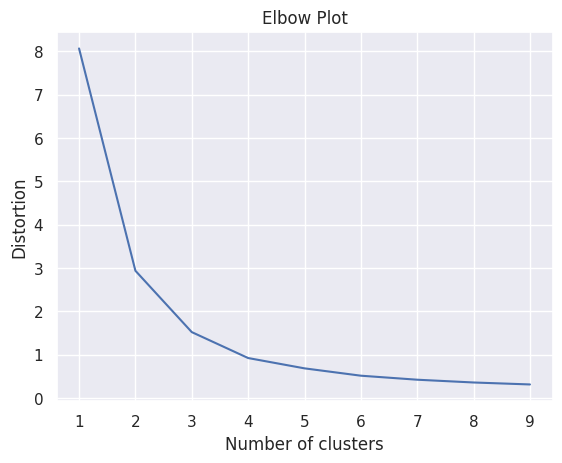
\includegraphics[width=\textwidth]{figures/tskmeans_elbow_b.png}
        \caption{Magnetic Field ($B$).}
        \label{fig:elbow_b}
    \end{subfigure}
    \hfill
    \begin{subfigure}[h]{0.48\textwidth}
        \centering
        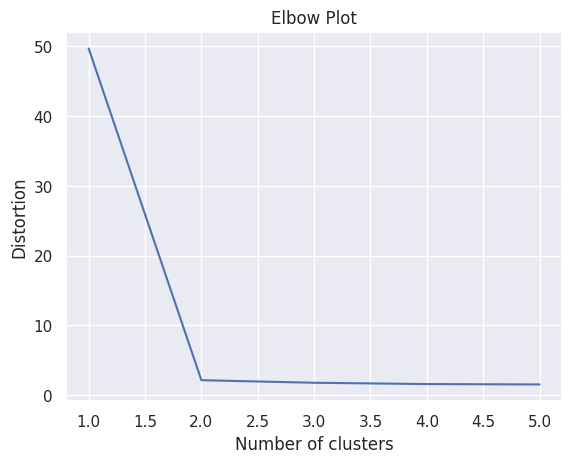
\includegraphics[width=\textwidth]{figures/tskmeans_elbow_alpha.png}
        \caption{Flux-tube inclination ($\alpha$).}
        \label{fig:elbow_alpha}
    \end{subfigure}
\end{figure}

\begin{table}[h]
    \caption[Validity Scores for TimeSeriesKmeans]{Validity metrics for different TimeSeriesKMeans models obtained by varying the number of clusters.}
    \begin{subtable}[h]{0.48\textwidth}
        \centering
        \begin{tabular}{@{}cccc@{}}
            \toprule
            \textbf{K} & \textbf{S score} & \textbf{DB} & \textbf{CH} \\ \midrule
            2          & 0.524               & 0.669                   & 20376                  \\
            3          & 0.511               & 0.628                   & 25585                  \\
            4          & 0.498               & 0.606                   & 30677                  \\
            5          & 0.458               & 0.648                   & 31995                  \\
            6          & 0.449               & 0.671                   & 34394                  \\
            7          & 0.431               & 0.695                   & 35462                  \\
            8          & 0.422               & 0.712                   & 36070                  \\
            9          & 0.403               & 0.738                   & 36368                  \\ \bottomrule
        \end{tabular}
        \caption{Magnetic Field ($B$)}
        \label{tab:tskmeans_b}
    \end{subtable}
    \hfill
    \begin{subtable}[h]{0.48\textwidth}
        \centering
        \begin{tabular}{@{}cccc@{}}
            \toprule
            \textbf{K} & \textbf{S score} & \textbf{DB} & \textbf{CH} \\ \midrule
            2          & 0.865               & 0.190                   & 263222                 \\
            3          & 0.499               & 1.078                   & 160481                 \\
            4          & 0.493               & 1.089                   & 120114                 \\
            5          & 0.463               & 1.123                   & 93537                  \\
            6          & 0.480               & 1.104                   & 82431                  \\
            7          & 0.259               & 1.312                   & 82038                  \\
            8          & 0.257               & 1.306                   & 76633                  \\
            9          & 0.252               & 1.374                   & 70313                  \\ \bottomrule
            \end{tabular}
        \caption{Flux-tube inclination ($\alpha$)}
        \label{tab:tskmeans_alpha}
    \end{subtable}
\end{table}


The elbow test for the magnetic field variable can be seen in Figure \ref{fig:elbow_b}. From this plot, it can be seen that the elbow is at $k=4$, which indicates that the optimal number of clusters is 4. However, this is not a clear elbow, as the curve is not smooth and the elbow is not very pronounced. This indicates that the optimal number of clusters is not very clear and that the results might not be very good.

To get a more precise number of clusters the validity metrics discussed in Section \ref{sec:validity_measures} were calculated for different KMeans models obtained by varying the number of clusters. The results of these tests can be seen in Table \ref{tab:tskmeans_b}. From the first three entries, it can be seen that the highest silhouette score is obtained with $K=2$, but the lowest Davies-Bouldin index is obtained with $k=4$, which also has the highest Calinski-Harabasz index of the three. This can serve as a possible indication that the correct number of clusters for this variable is 4.

Following the same procedure as for the magnetic field, an elbow test was conducted on the flux tube inclination variable, $\alpha$. The results of this test can be seen in Figure \ref{fig:elbow_alpha}. In contrast with the results of the previous test, this elbow is much clearer, with the elbow being at $k=2$. This indicates that the optimal number of clusters is 2.

The validity metrics (table \ref{tab:tskmeans_alpha}) also provide a clear indication that the correct number of clusters for this variable is 2, with the highest Silhouette and Calinski-Harabasz scores being obtained with $k=2$. The Davies-Bouldin index is also the lowest for this value.


\subsection{SOM}\label{sec:som_experiments}
Following the experiments with TimeSeriesKmeans, the SOM algorithm was tested, which is also seen as a useful method for clustering high-dimension data. A Python implementation of the algorithm \cite{vettigliminisom} was tested on the same variables as the previous algorithm, $B$ and $\alpha$. Unlike KMeans, this algorithm does not have any tests to visually determine the number of clusters. Because of this, the number of clusters was determined by trial and error, by varying the number of clusters and evaluating the results of the validity metrics (table \ref{tab:validity_som}). The first two columns of each subtable indicate the $x$ and $y$ dimensions of the SOM map used for the clustering task. The number of clusters is obtained by multiplying these two values.

\begin{table}[h]
    \caption[Validity Scores for SOM]{Validity metrics for different SOM models obtained by varying sizes of the maps ($x$ and $y$ variables).}\label{tab:validity_som}
    \begin{subtable}[h]{0.48\textwidth}
        \centering
        \begin{tabular}{@{}ccccc@{}}
            \toprule
            \textbf{x} & \textbf{y} & \textbf{S score} & \textbf{DB} & \textbf{CH} \\ \midrule
            2          & 2          & 0.500            & 0.602       & 30962   \\
            2          & 3          & 0.281            & 5.228       & 3429    \\
            3          & 2          & 0.454            & 0.660       & 35001   \\
            3          & 3          & 0.407            & 0.727       & 37133   \\ \bottomrule
            \end{tabular}
        \caption{Magnetic Field ($B$)}
        \label{tab:som_b}
    \end{subtable}
    \hfill
    \begin{subtable}[h]{0.48\textwidth}
        \centering
        \begin{tabular}{@{}ccccc@{}}
            \toprule
            \textbf{x} & \textbf{y} & \textbf{S score} & \textbf{DB} & \textbf{CH} \\ \midrule
            2          & 2          & 0.269            & 1.479       & 122195 \\
            2          & 3          & 0.004            & 1.325       & 5254    \\
            3          & 2          & 0.269            & 1.326       & 89759   \\
            3          & 3          & 0.231            & 1.426       & 66878   \\ \bottomrule
            \end{tabular}
        \caption{Flux-tube inclination ($\alpha$)}
        \label{tab:som_alpha}
    \end{subtable}
\end{table}

From looking at the results of the validity metrics for the magnetic field variable (table \ref{tab:som_b}), it can be concluded that the highest Silhouette score and DB index are obtained with $x=2$ and $y=2$, which translate to 4 clusters. For a map size of $x=2$ and $y=3$, the algorithm completely failed to generate a proper separation. The Calinski-Harabasz index is the highest for $x=3$ and $y=3$, which translates to 9 clusters. However, this is not a clear indication that this is the correct number of clusters, as the DB index is higher than the first clustering.

The results of the validity metrics for the flux tube inclination variable (table \ref{tab:som_alpha}) are even less clear than the previous ones. The highest Silhouette score is obtained with the first and third models. The best CH index was by far the first one. The DB index is very high for every model that was generated, which indicates that clustering in this variable may not be a good idea.

Overall the results from this experiment indicate that the SOM algorithm is not a good choice for clustering this dataset, as it is not able to generate a clear separation between the clusters. This is especially true for the flux tube inclination variable, where the algorithm completely failed to generate a proper separation. The only variable where the algorithm was able to generate a somewhat clear separation was the magnetic field with a map of 2x2 neurons.


\subsection{PCA Clustering Approach}\label{sec:pca_clustering}
The next approach that was tested was to apply PCA to the dataset and then apply the clustering algorithms to the reduced dataset. This approach was tested on the magnetic field variable, $B[G]$, the flux tube inclination, $\alpha [deg]$, and lastly on a combination of all the input variables. 

Tests were conducted to try and find the optimal number of components that would explain the dataset. This was done by analyzing the cumulative explained variance of PCA models with different \textit{n\_components}. For $B$ and $\alpha$ about 99\% of the variance was explained by just 2 components. As for the combined dataset, 98\% was explained by also 2 components. With this, it can be concluded that it is valid to reduce the dimensionality of this dataset to just two components. This is useful because it provides a simplified representation of the data while preserving most of the information. 

The representations for each of the approaches can be seen in Figure \ref{fig:pca_mag_2d}. Note that the representation generated for the flux-tube indication and the joint inputs are very similar. This indicates that the flux-tube inclination variable is the one that contributes the most to the PCA.

For the clustering part, the KMeans and the AgglomerativeClustering methods of the \textit{sklearn} library were applied to each of the representations to determine the correct number of clusters with the same methodology as in the previous sections. 

\begin{figure}[h]
    \caption[PCA applied to the different variables]{PCA applied to the different variables. (a) and (b) represent the PCAs of the magnetic field variable ($B[G]$) and the flux-tube inclination variable ($\alpha [deg]$), respectively; (c) is the PCA of all input variables combined.}
    \label{fig:pca_mag_2d}
    \begin{subfigure}[h]{0.329\textwidth}
        \centering
        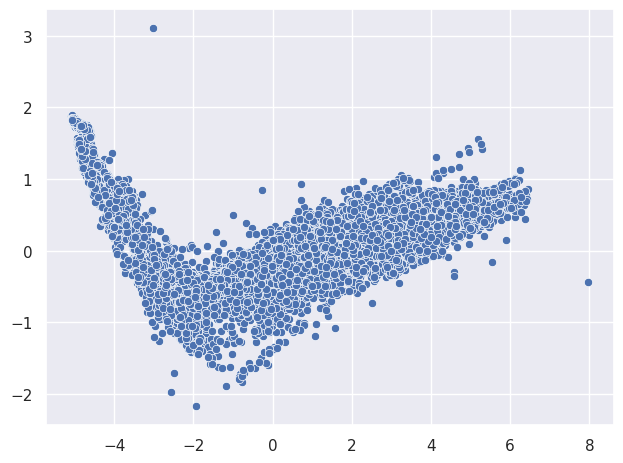
\includegraphics[width=\textwidth]{figures/mag_pca_2d.png}
        \caption{Magnetic Field ($B$).}
        \label{fig:pca_mag_2d}
    \end{subfigure}
    \hfill
    \begin{subfigure}[h]{0.329\textwidth}
        \centering
        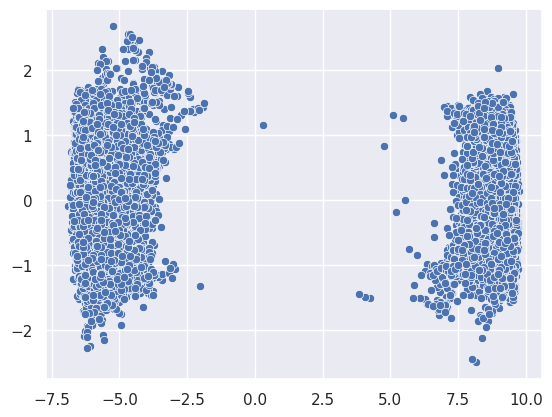
\includegraphics[width=\textwidth]{figures/alpha_pca_2d.png}
        \caption{Flux-tube inclination ($\alpha$).}
        \label{fig:pca_alpha_2d}
    \end{subfigure}
    \begin{subfigure}[h]{0.329\textwidth}
        \centering
        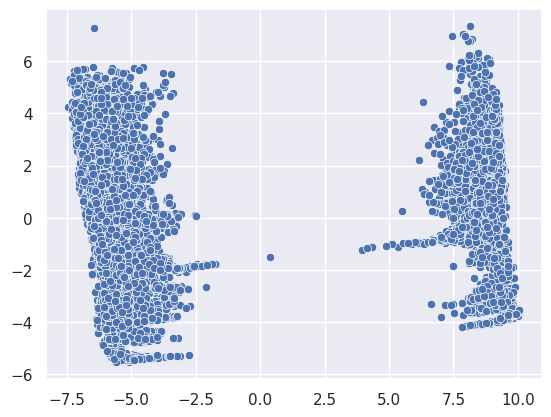
\includegraphics[width=\textwidth]{figures/pca_joint_2d.png}
        \caption{Joint Inputs ($R$, $B$ and $\alpha$).}
        \label{fig:pca_joint_2d}
    \end{subfigure}
\end{figure}

% \begin{figure}
%     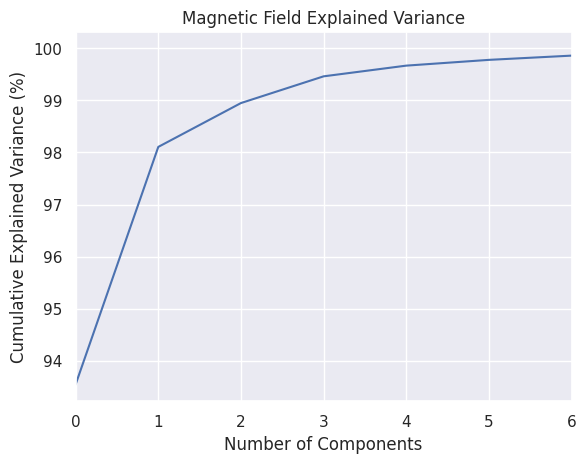
\includegraphics{figures/pca_mag_explained_variance.png}
%     \caption{Explained variance for the PCA of the magnetic field variable.}
% \end{figure}

\subsubsection{PCA of the Magnetic Field}\label{sec:pca_b}

The KMeans and the AgglomerativeClustering methods were applied to the PCA of the magnetic field variable. The results of the elbow tests for KMeans can be seen in Figure \ref{fig:pca_b_elbow}. From this plot, it can be seen that the elbow is at $k=4$, which is an indication that the optimal number of clusters might be 4. 

\begin{figure}
    \caption{KMeans Elbow test for the PCA of the magnetic field variable.}
    \label{fig:pca_b_elbow}
    \centering
    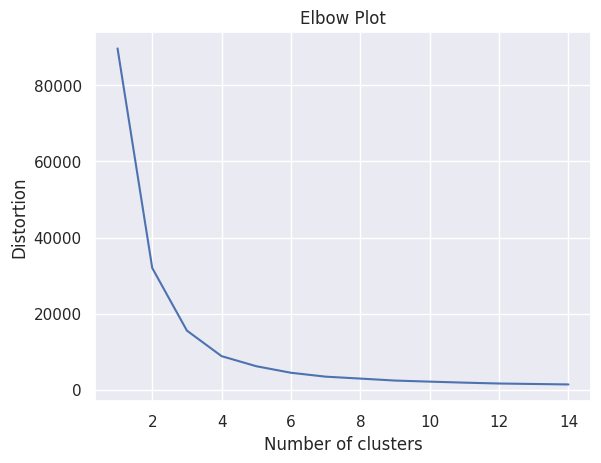
\includegraphics[width=0.6\textwidth]{figures/pca_mag_elbow_test.png}
\end{figure}

To get a more concrete outlook, the validity measures from the previous sections were calculated for each of the methods. The results of these tests can be seen in Table \ref{tab:pca_b}. For the KMeans algorithm, the highest Silhouette score is obtained with $K=2$, but the lowest Davies-Bouldin index is obtained with $K=4$, which also has the highest Calinski-Harabasz index of the first three results. This further confirms the results of the elbow test. 

The results of the Agglomerative method are not as clear as the previous ones. The highest silhouette score is also with $K=2$, but as in Kmeans, the lowest DB index was with $K=4$. In addition, the CH score is much higher for the model with 4 clusters than for the $K=2$ model.


% Please add the following required packages to your document preamble:
% \usepackage{booktabs}
\begin{table}[h]
    \caption[Validity metrics for PCA of the Magnetic Field]{Validity metrics obtained by different clustering methods on the PCA of the magnetic field variable. Various models were created for each method by varying the number of clusters, $K$.}\label{tab:pca_b}
    \begin{tabular}{@{}rrrrccc@{}}
        \toprule
    \multicolumn{1}{c}{\textbf{}}   & \multicolumn{3}{c}{\textbf{KMeans}}                                                                       & \multicolumn{3}{c}{\textbf{Agglomerative}}   \\ \midrule
    \multicolumn{1}{c|}{\textbf{K}} & \multicolumn{1}{c}{\textbf{S score}} & \multicolumn{1}{c}{\textbf{DB}} & \multicolumn{1}{c|}{\textbf{CH}} & \textbf{S score} & \textbf{DB} & \textbf{CH} \\ \midrule
    \multicolumn{1}{r|}{2}          & 0.538                                & 0.645                           & \multicolumn{1}{r|}{21224}   & 0.507            & 0.669       & 17899   \\
    \multicolumn{1}{r|}{3}          & 0.534                                & 0.586                           & \multicolumn{1}{r|}{28086}   & 0.496            & 0.622       & 23868   \\
    \multicolumn{1}{r|}{4}          & 0.531                                & 0.549                           & \multicolumn{1}{r|}{35942}   & 0.502            & 0.550       & 30612   \\
    \multicolumn{1}{r|}{5}          & 0.502                                & 0.579                           & \multicolumn{1}{r|}{39762}   & 0.484            & 0.593       & 37737   \\
    \multicolumn{1}{r|}{6}          & 0.494                                & 0.592                           & \multicolumn{1}{r|}{44986}   & 0.477            & 0.585       & 40121   \\
    \multicolumn{1}{r|}{7}          & 0.486                                & 0.600                           & \multicolumn{1}{r|}{49233}   & 0.460            & 0.598       & 44158   \\
    \multicolumn{1}{r|}{8}          & 0.454                                & 0.637                           & \multicolumn{1}{r|}{49757}   & 0.436            & 0.638       & 45487   \\
    \multicolumn{1}{r|}{9}          & 0.457                                & 0.636                           & \multicolumn{1}{r|}{53265}   & 0.427            & 0.630       & 47528   \\ \bottomrule
    \end{tabular}
    \end{table}

With the consensus of both clustering methods, it can be concluded that the optimal number of clusters for the PCA of the magnetic field variable is 4. Interestingly, this is the same number of clusters that were obtained with the TimeSeriesKMeans algorithm in Section \ref{sec:time_series_methods} and the SOM algorithm in Section \ref{sec:som_experiments} for the magnetic field.

\subsubsection{PCA of the Flux-tube Inclination}\label{sec:pca_a}
Following the same procedure as in the approach, an elbow test was conducted for the KMeans model of the PCA of the flux-tube inclination variable. The results of this test can be seen in Figure \ref{fig:pca_a_elbow}. The plot indicates that the most appropriate number of clusters is 2.


\begin{figure}[h]
    \caption{KMeans Elbow test for the PCA of the flux-tube inclination variable.}
    \label{fig:pca_a_elbow}
    \centering
    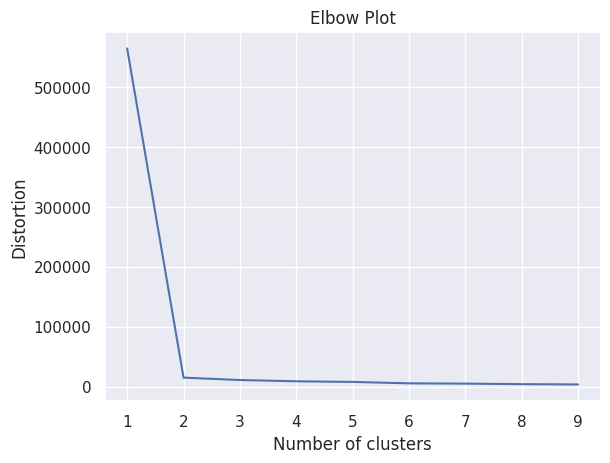
\includegraphics[width=0.6\textwidth]{figures/pca_alpha_elbow_test.png}
\end{figure}

These results are further corroborated by the validity metrics in Table \ref{tab:pca_a}. The highest Silhouette score and DB index are obtained with $K=2$, which also has the highest Calinski-Harabasz index of all the results. This indicates that the optimal number of clusters is 2, for both of the tested methods. This division occurs because the $\alpha$ variable may take negative or positive values.

\begin{table}[h]
    \caption[Validity metrics for PCA of the Flux-tube Inclination]{Validity metrics obtained by different clustering methods on the PCA of the flux-tube inclination variable. Various models were created for each method by varying the number of clusters, $K$.}\label{tab:pca_a}
    \begin{tabular}{@{}cccc|ccc@{}}
    \toprule
    \multicolumn{1}{l}{}            & \multicolumn{3}{c|}{\textbf{KMeans}}         & \multicolumn{3}{c}{\textbf{Agglomerative}}   \\ \midrule
    \multicolumn{1}{c|}{\textbf{K}} & \textbf{S score} & \textbf{DB} & \textbf{CH} & \textbf{S score} & \textbf{DB} & \textbf{CH} \\ \midrule
    \multicolumn{1}{c|}{2}          & 0.898            & 0.145       & 428761  & 0.898            & 0.145       & 428761  \\
    \multicolumn{1}{c|}{3}          & 0.586            & 0.757       & 294424  & 0.574            & 0.782       & 287595  \\
    \multicolumn{1}{c|}{4}          & 0.593            & 0.662       & 243422  & 0.378            & 1.022       & 239082  \\
    \multicolumn{1}{c|}{5}          & 0.583            & 0.713       & 207238  & 0.354            & 0.955       & 219099  \\
    \multicolumn{1}{c|}{6}          & 0.400            & 0.887       & 237197  & 0.359            & 0.924       & 215351  \\
    \multicolumn{1}{c|}{7}          & 0.392            & 0.917       & 216689  & 0.360            & 0.900       & 211272  \\
    \multicolumn{1}{c|}{8}          & 0.391            & 0.875       & 225758  & 0.338            & 0.906       & 199083  \\
    \multicolumn{1}{c|}{9}          & 0.381            & 0.901       & 223637  & 0.336            & 0.890       & 189224  \\ \bottomrule
    \end{tabular}
    \end{table}

\subsubsection{PCA of the Joint Inputs}\label{sec:pca_joint}



\section{Results}\label{sec:clustering_results}

\chapter{Conclusions} \label{chap:conclusion}

The necessity to consistently predict the Sun's conditions that lead to the most extreme events has become an increasingly important study. However, technological difficulties make it challenging to obtain real-time data from the Sun's surface. Multiple numeric simulators have tried to fill this gap by extrapolating these conditions based on limited observations from Earth. In this dissertation, we have explained the problems (sec. \ref{sec:prob_definition}) associated with these solutions that severely affect the ability to generate solar estimations promptly. These issues included the long execution time of the simulation models as well as the need for initial expert estimations. Additionally, it was posited that the use of machine learning techniques to predict the original conditions suffered greatly from anomalies in the training dataset.

To address these issues, we first studied the current most popular GAN-based techniques for anomaly detection. The state-of-the-art analysis (sec. \ref{sec:stoa_results}) showed that GAN-based anomaly detection techniques performed the task better than other mainstream methods. With this in mind, we proposed a GAN-based anomaly detection technique (sec. \ref{sec:method}) that detects anomalies in the training dataset used by the prediction models. In the same section, the evaluation methods that will be used for the validation of the results were also explained. Finally, the work plan (sec. \ref{sec:work_plan}) was presented, which included the tasks that will be performed to achieve the objectives of the dissertation.






%%----------------------------------------
%% Final materials
%%----------------------------------------

%% Bibliography
%% Comment the next command if BibTeX file not used
%% bibliography is in ``myrefs.bib''
\PrintBib{myrefs}

%% 2021-07-20: change
%% comment next 2 commands if numbered appendices are not used
\appendix




%% Index
%% Uncomment next command if index is required
%% don't forget to run ``makeindex thesis'' command
%\PrintIndex

\end{document}
